\section{Newton's bewegingswetten}

\vspace{0.5cm}

\begin{theo}[Kracht]{Kracht}

Een kracht is een actie die de snelheid van een voorwerp verandert. Elke versnelling wordt dus veroorzaakt door een kracht. Er zijn twee soorten krachten: 

\begin{itemize}
    \item \textbf{Contactkrachten:} fysisch contact vindt plaats
    \item \textbf{Veldkrachten:} werken op een zekere afstand
\end{itemize}

\hspace{-0.65cm} Een kracht is een vectoriële grootheid en heeft dus een grootte, richting en zin.

\end{theo}

\begin{lem}[De eerste wet van Newton: de Inertiewet]{De eerste wet van Newton: de Inertiewet}

Een lichaam in rust (of in eenparige rechtlijnige beweging) zal in rust (eenparige rechtlijnige beweging) blijven tenzij er een uitwendige resulterende kracht inwerkt

    \begin{equation*}
        \sum_{i} \Vec{F}_i = 0 \to \Vec{a} = 0
    \end{equation*}

\hspace{-0.65cm} Een \textbf{inertiaalstelsel} is een referentiestelsel waarin de eerste wet van Newton geldt. De \textbf{inertie} wordt gegeven door de massa en beschrijft hoeveel weerstand dat een lichaam biedt tegen een verandering van zijn snelheid. 

    % \begin{equation*}
    %     \dfrac{m_1}{m_2} = \dfrac{a_2}{a_1}
    % \end{equation*}

\end{lem}

\begin{lem}[De tweede wet van Newton: de versnellingswet]{De tweede wet van Newton: de versnellingswet}

De versnelling van een voorwerp is recht evenredig met de nettokracht op het voorwerp en omgekeerd evenredig met het massa van het voorwerp. De richting van de versnelling is dezelfde als de richting van de nettokracht.

    \begin{equation*}
        \sum_{i} \Vec{F}_i = \Vec{F}_{net} = m\Vec{a} = m\dfrac{d\Vec{v}}{dt} = m\dfrac{d^2\Vec{r}}{dt^2}
    \end{equation*}

\end{lem}

\begin{lem}[De derde wet van Newton: de actie-reactiewet]{De derde wet van Newton: de actie-reactiewet}

Wanneer een voorwerp een kracht uitoefent op een ander voorwerp, dan oefent het ander voorwerp een kracht met dezelfde grootte en omgekeerde zin uit op het voorwerp.

    \begin{align*}
        \Vec{F}_{1 \to 2} &= -\Vec{F}_{2 \to 1} \\
       F_{1 \to 2} &= F_{2 \to 1}
    \end{align*}

\end{lem}

\newpage

\begin{theo}[Gravitatiekracht]{Gravitatiekracht}
Alle voorwerpen nabij het aardoppervlak vallen met dezelfde versnelling $ \Vec{g} $. De kracht bepaald door deze versnelling wordt de \textbf{gravitatiekracht} of \textbf{zwaartekracht} genoemd:

    \begin{equation*}
        \Vec{F}_G = m\Vec{g}
    \end{equation*}

\noindent Deze kracht is gericht naar het aardoppervlak toe en de grootte wordt het \textbf{gewicht} van een voorwerp genoemd. 

\end{theo}

\begin{theo}[Normaalkracht]{Normaalkracht}
    De \textbf{loodrechte} kracht die het contactoppervlak uitoefent op het voorwerp 
    \begin{equation*}
        F_N = F_{g,y} - \sum_{rest,y} F_{rest,y}
    \end{equation*}
    \noindent wordt de normaalkracht genoemd. De volgende figuren tonen enkele veelvoorkomende situaties voor de oefeningen:
    
    \begin{minipage}{.48\textwidth}
    
        \centering
        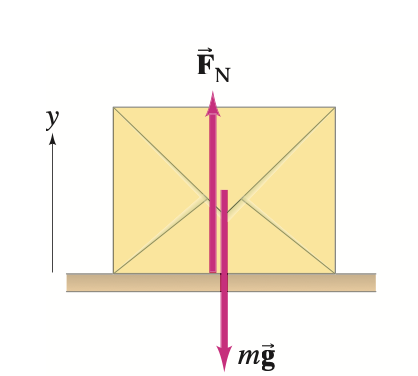
\includegraphics[scale = 0.7]{Images/Dynamica/Doos in rust.png}   
    
    \end{minipage} 
    \begin{minipage}{.48\textwidth}
    
        \centering
        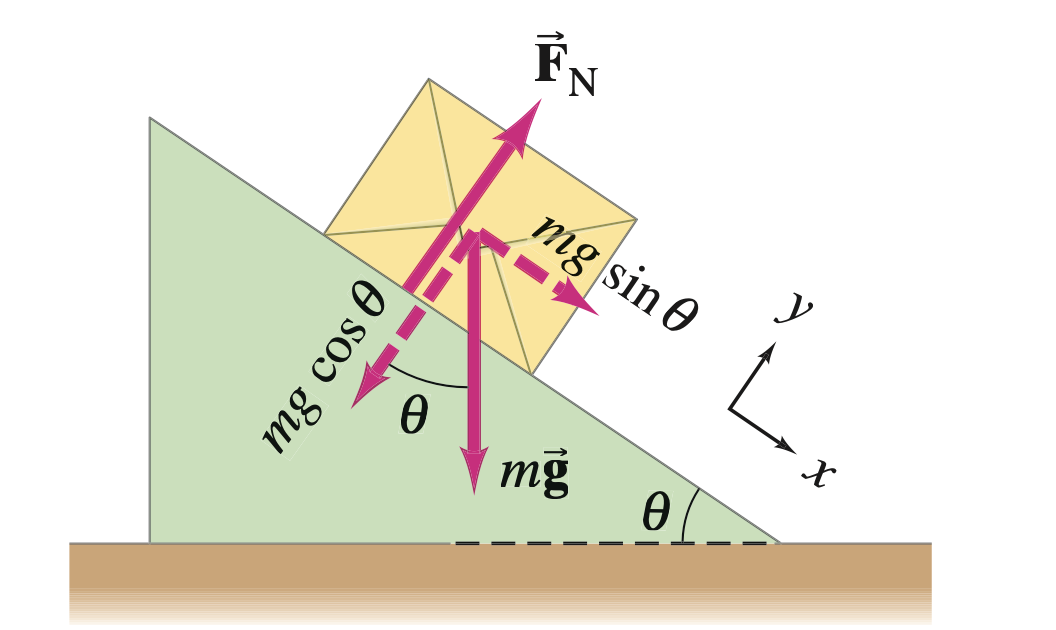
\includegraphics[scale = 0.35]{Images/Dynamica/Glijdende doos.png}
        
    \end{minipage}
    
    \vspace{0.25cm}
    
    \noindent De normaalkracht is dus afhankelijk van de gravitatiekracht van zijn grootte en zin, maar niet van zijn richting (zie de rechtse figuur). We kunnen dus \textbf{niet} zeggen dat het gravitatiekracht-normaalkracht paar een actie-reactie paar vormt. 
\end{theo}




\newpage

\section{De wetten van Newton: wrijving, cirkelbeweging, weerstandskrachten}

\vspace{0.5cm}

\begin{theo}[Wrijvingskracht]{Wrijvingskracht}

    De wrijvingkracht is de weerstand die het voorwerp ondervindt wanneer het over het oppervlak van een ander voorwerp beweegt. We bespreken 2 soorten wrijvingskrachten:
    
    \begin{itemize}
        \item \textbf{Kinetische:} $ F_k = \mu_kF_N$ met $ \mu_k $ de \textbf{kinetische} wrijvingscoëffiënt. Deze kracht is recht evenredig met de normaalkracht.
        \item \textbf{Statische:} $ F_s \leq \mu_sF_N$ met $ \mu_s $ de \textbf{statische} wrijvingscoëffiënt. Als deze drempelwaarde bereikt is, dan zal het object beginnen met bewegen en zal er sprake zijn van kinetische wrijving.
    \end{itemize}
    
    \noindent Er geldt dat het moeilijker is om een voorwerp te laten starten dan om een beweging verder te laten verlopen, of in formule vorm: 
    
    \vspace{-0.2cm}
    \begin{equation*}
        \mu_s > \mu_k
    \end{equation*} 
    \vspace{-0.4cm}
\end{theo}

% \begin{ex}[Voorbeeld: Wrijvingskracht]{Voorbeeld: Wrijvingskracht1}
%         \centering
%         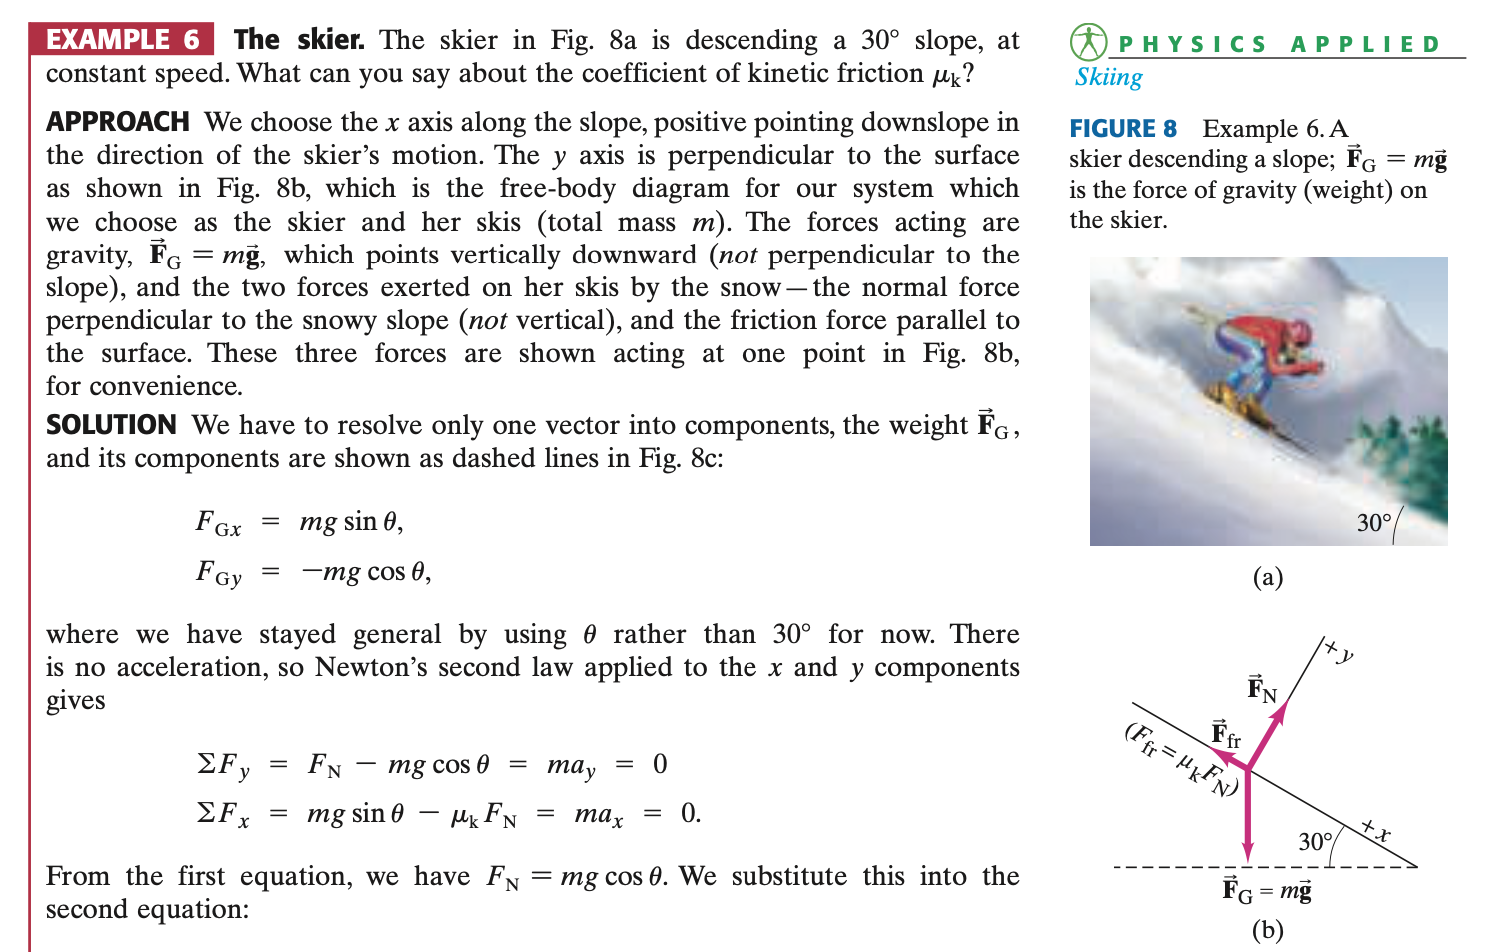
\includegraphics[scale = 0.6]{Examples/Dynamica/5.6.1.png}
%         \centering
%         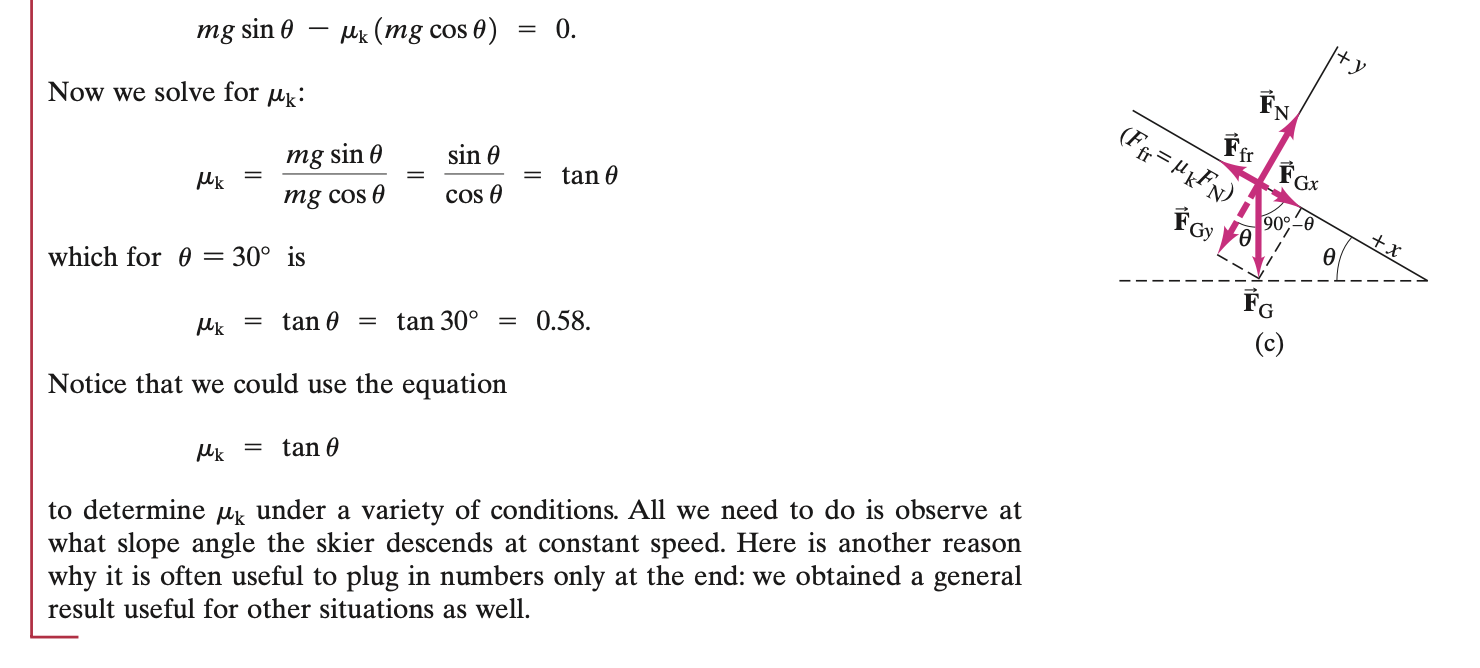
\includegraphics[scale = 0.6]{Examples/Dynamica/5.6.2.png}
%         \vspace{-0.5cm}
% \end{ex}

\begin{theo}[Kinematica van de eenparige cirkelbeweging]{Kinematica van de eenparige cirkelbeweging}
    \vspace{-0.4cm}
    \begin{minipage}{.71\textwidth}
        % We berekenen de versnelling door te vertrekken van de formule:
        % \begin{equation}
        %     \Vec{a} = \lim_{\Delta t \to 0} \dfrac{\Delta \Vec{v}}{\Delta t} = \dfrac{d\Vec{v}}{dt}
        % \end{equation}
        Een voorwerp dat met een constante snelheid in een cirkel beweegt voert een \textbf{eenparig cirkelvormige beweging} uit. In dit soort beweging blijft de grootte van de snelheidsvector constant, maar verandert de richting continu, m.a.w. $ a \neq 0 $. Uit gelijkvormige driehoeken volgt: 
    
        \begin{equation*}
            \dfrac{\Delta v}{v} \approx \dfrac{\Delta \ell}{r} \to \Delta v \approx \dfrac{v}{r}\Delta \ell
        \end{equation*}

        % \begin{center}
        %     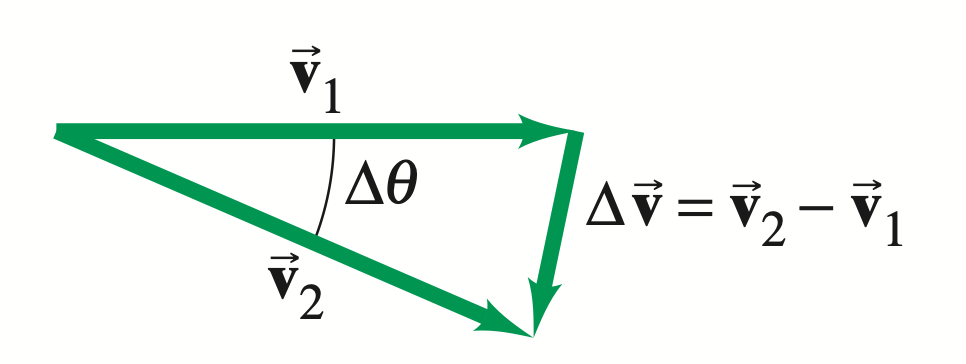
\includegraphics[scale = 0.25]{Images/Dynamica/Gelijkvormige driehoeken stap.png}
        % \end{center}
        
        \noindent en hiermuit kunnen we de middelpuntzoekende versnelling berekenen
        \begin{equation*}
            a_R = \lim_{\Delta t \to 0} \frac{\Delta v}{\Delta t} = \lim_{\Delta t \to 0} \frac{v}{r}\frac{\Delta \ell}{\Delta t} = \frac{v^2}{r}
        \end{equation*}
    \end{minipage} 
    \begin{minipage}{.25\textwidth}
        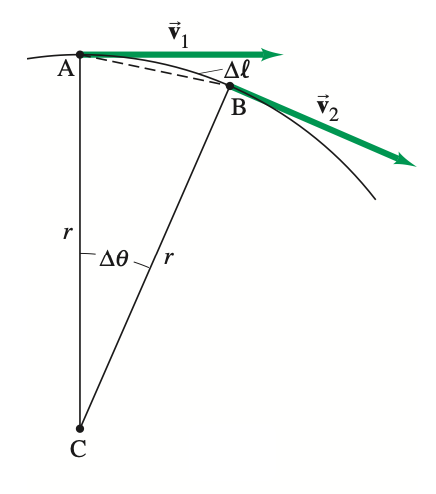
\includegraphics[scale = 0.3]{Images/Dynamica/Kinematica van de Cirkelbeweging.png}      
    \end{minipage}
    \vspace{0.3cm}

    \noindent Deze versnelling wordt de \textbf{centripetale versnelling} genoemd en is gericht naar het middelpunt van de cirkel. De snelheid van een ECB wordt gegeven door de volgende formule: 
    \begin{equation*}
        v = \dfrac{2\pi r}{T}
    \end{equation*}
    \noindent Hierbij is T de periode, m.a.w. tijd nodig voor een complete omwenteling. De frequentie van de ECB, m.a.w het aantal omwentelingen per seconde, wordt gegeven door de volgende formule
    \begin{equation*}
        f = \dfrac{1}{T} = \dfrac{v}{2\pi r} = \dfrac{\omega}{2\pi}
    \end{equation*}
    waarbij de dimensie Hz is.
\end{theo}

\newpage

\begin{theo}[Dynamica van de eenparige cirkelbeweging]{Dyamica van de eenparige cirkelbeweging}
    De cirkelbeweging is een versnelde beweging, dus er is een resulterende kracht nodig om het voorwerp op de cirkelbaan te houden, namelijk de \textbf{centripetale kracht}:

    \begin{equation*}
        (\sum F)_R = ma_R = m\dfrac{v^2}{r}
    \end{equation*}
    
    \noindent Om een voorwerp op een cirkelbaan te houden is er een centripetale versnelling en zoals hierboven vermeld een centripetale kracht nodig, dus de $ F_{net} $ moet naar het midden van de cirkel gericht zijn. Als deze kracht er niet is, dan zal het volgens de \textbf{Inertiewet} rechtlijnig zich voortbewegen.
\end{theo}
 
\begin{theo}[Kinematica én Dynamica niet-eenparige cirkelbeweging]{Niet-eenparige cirkelbeweging}
    In dit soort beweging beweegt het voorwerp volgens een cirkelbaan, maar kan het versnellen. De totale vectoriele versnelling in dit soort beweging wordt gegeven door de volgende formule:
    \begin{equation*}
        \Vec{a} = \Vec{a}_{tan} + \Vec{a}_R 
    \end{equation*}

    \noindent Sinds $ \Vec{a}_R $ en $ \Vec{a}_{tan} $ altijd loodrecht op elkaar staan, geldt op eenderwelk ogenblik:
        \begin{equation*}
            a = \sqrt{a_{tan}^2 + a_R^2} \text{ met } a_R = \dfrac{v^2}{r} \text{ en } a_{tan} = \dfrac{dv}{dt}
        \end{equation*}

    \noindent De figuren tonen de tangentiele en centripetale krachten en versnellingen bij een niet-eenparige cirkelbeweging:
    
        \begin{center}
            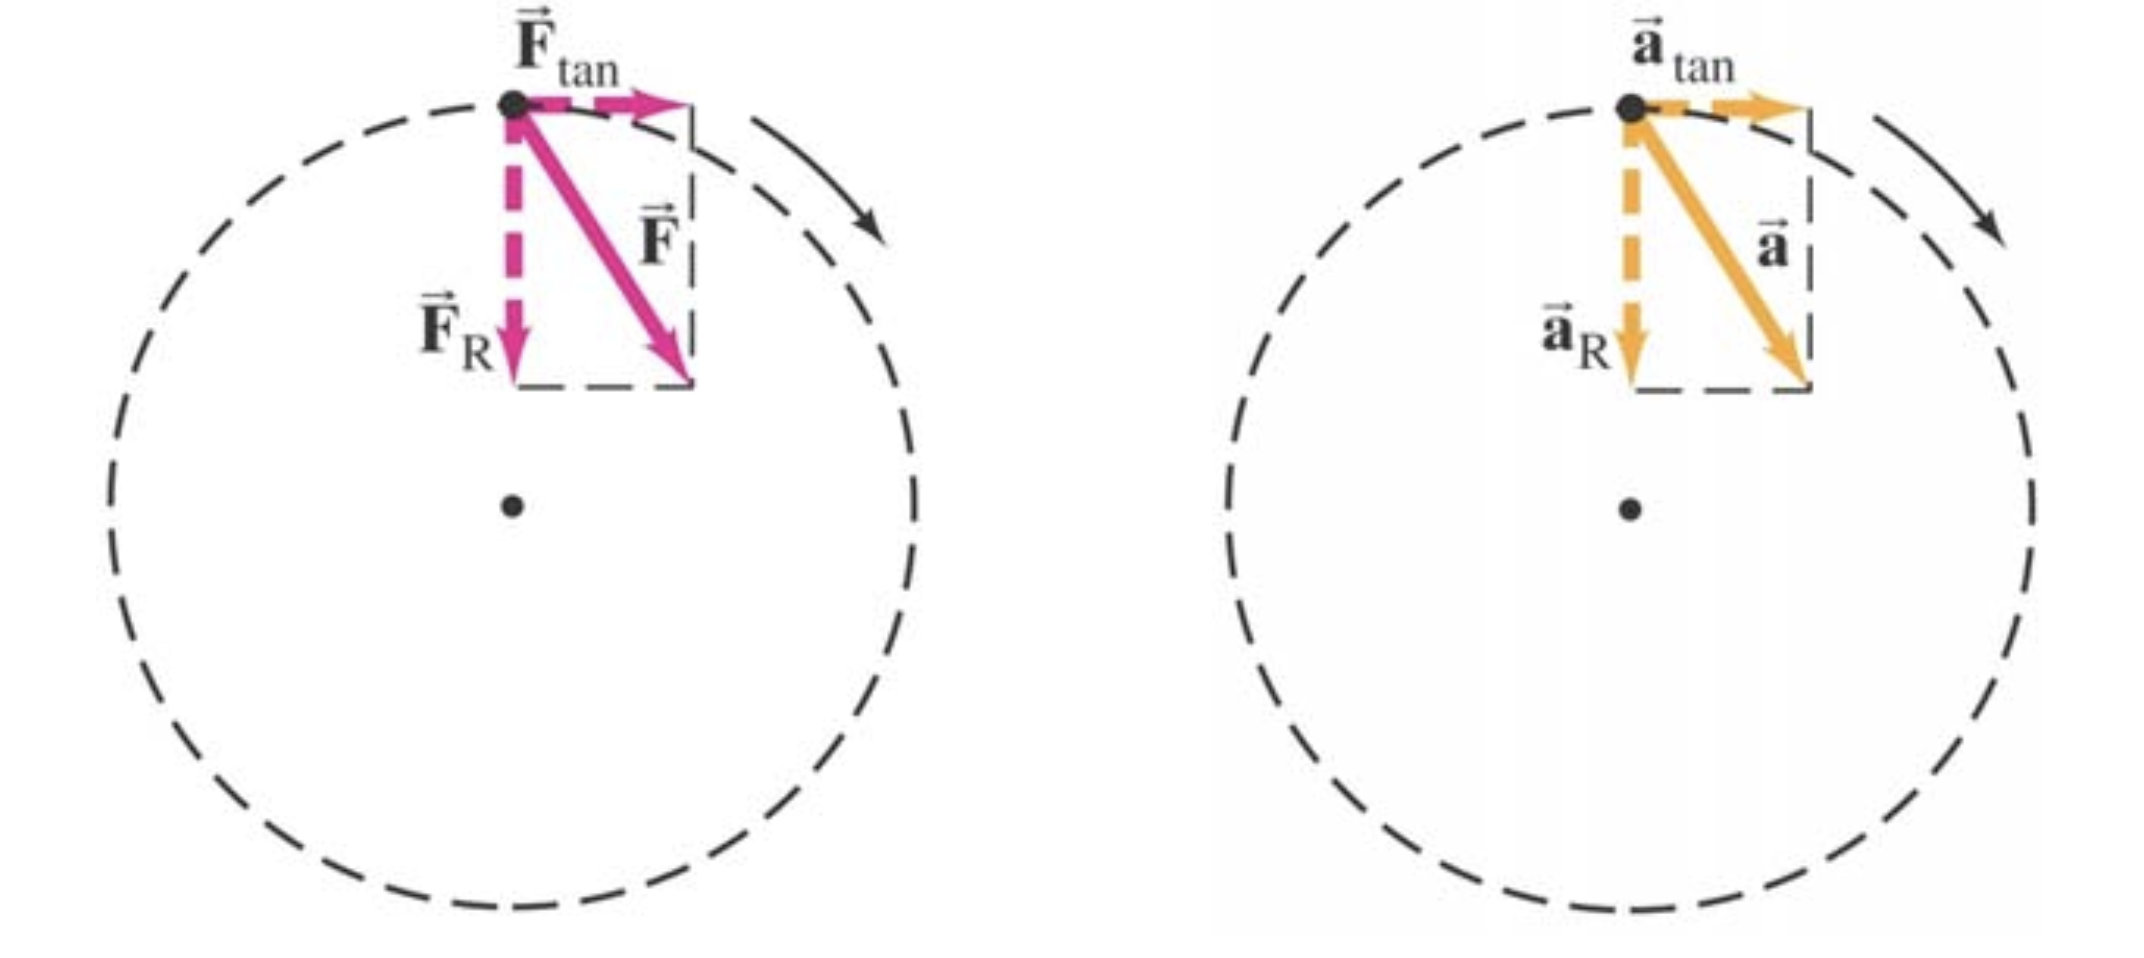
\includegraphics[scale = 0.20]{Images/Dynamica/Niet-Eenparige Cirkelbeweging.png} 
        \end{center}
\end{theo}

% \begin{ex}[Voorbeeld: Eenparige cirkelbeweging]{Eenparige cirkelbeweging}
%     \centering
%     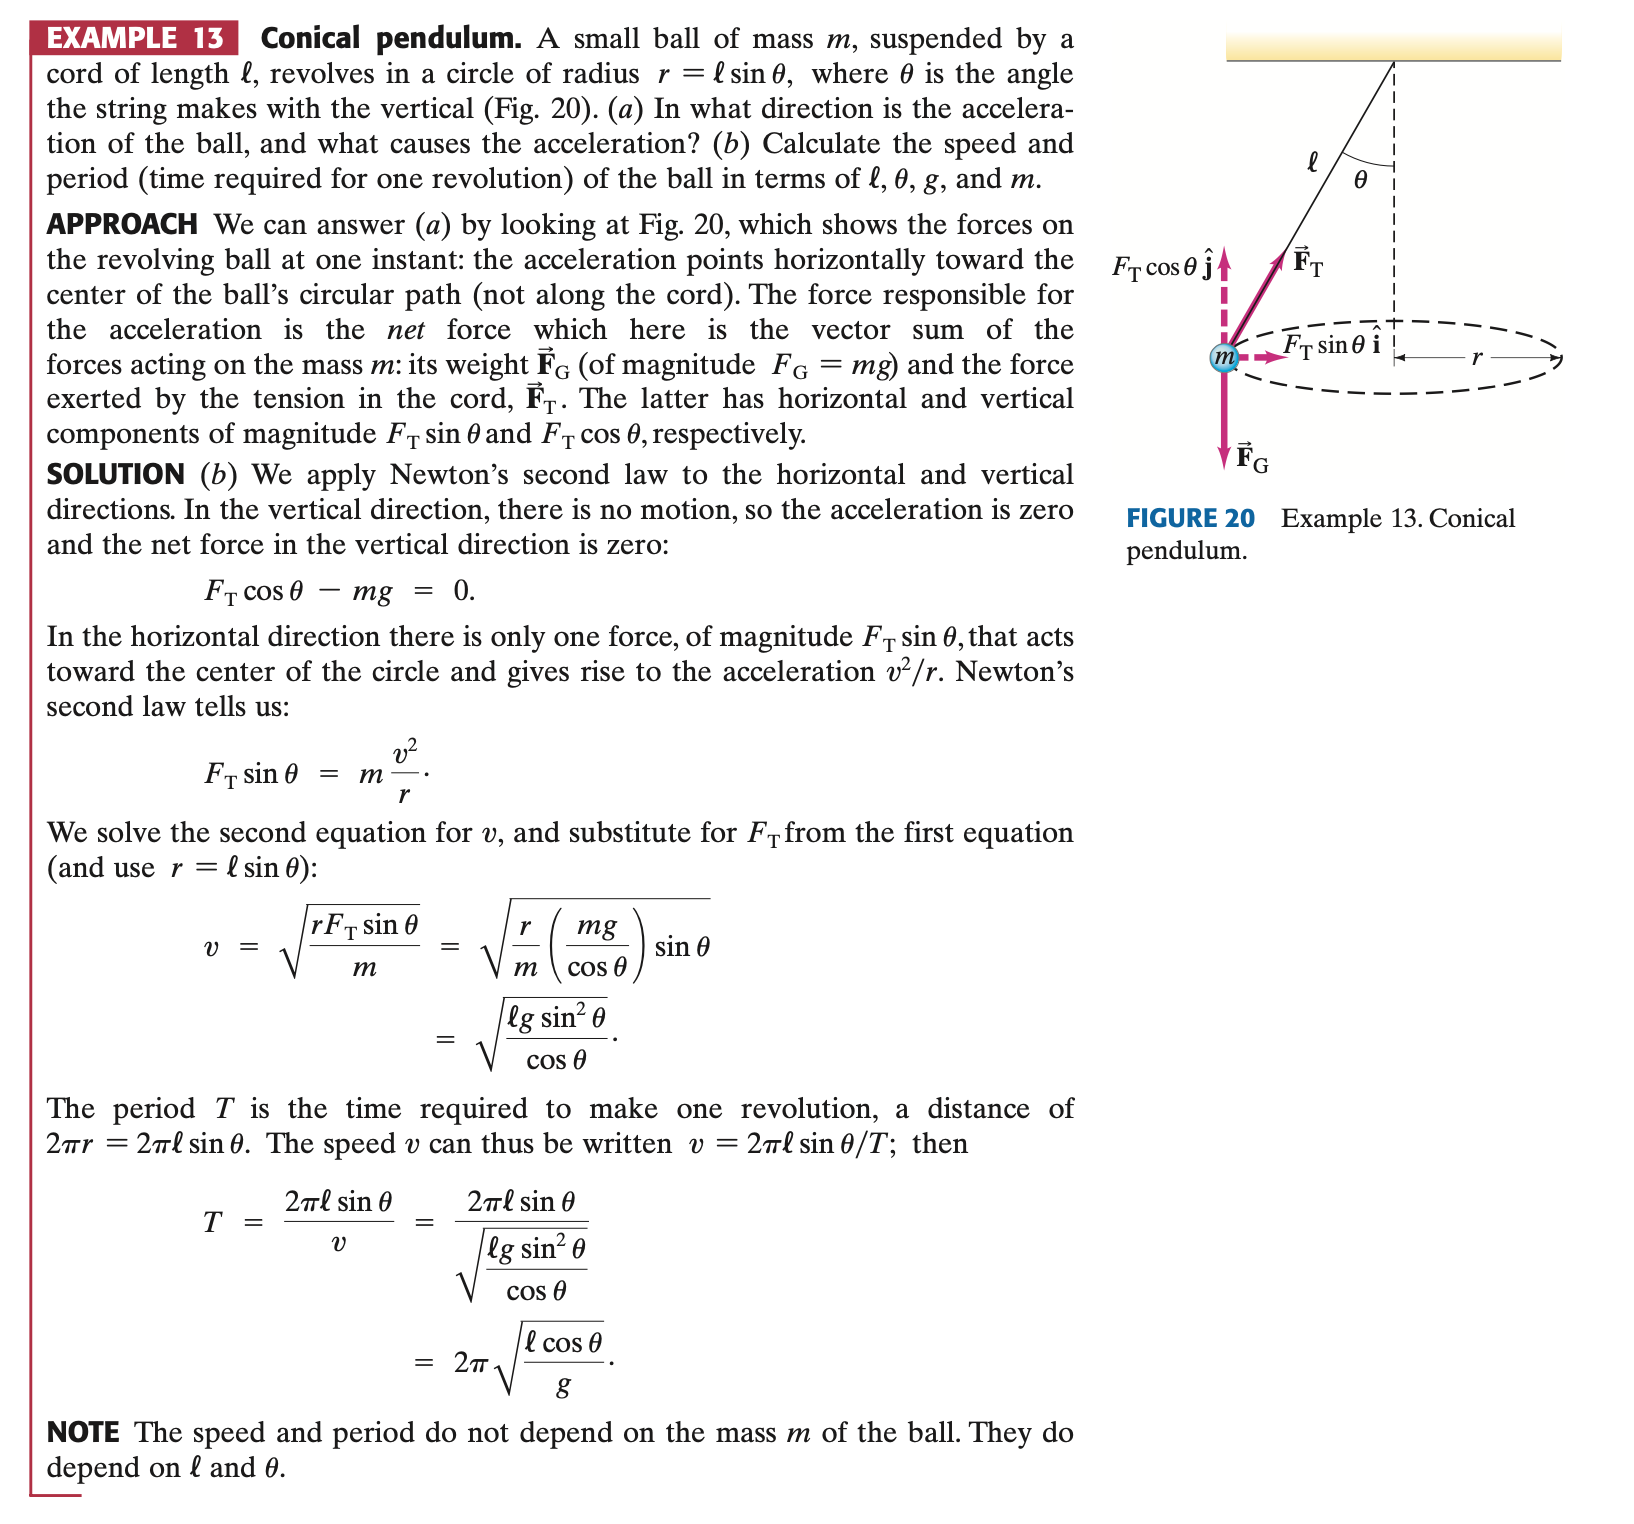
\includegraphics[scale = 0.55]{Examples/Dynamica/5.13.png}
% \end{ex}

\newpage

\section{De zwaartekracht en de synthese van Newton}

\vspace{0.5cm}

\begin{theo}[De wet van de universele zwaartekracht]{De wet van de universele zwaartekracht}

Elk deeltje in het heelal trekt elk ander deeltje aan met een kracht die recht evenredig is met het product van hun massa’s en omgekeerd evenredig met het kwadraat van de onderlinge afstand, in formulevorm:
 
 \begin{equation*}
     F_g = G\dfrac{m_1m_2}{r^2} \text{ met } G = 6.673 \times 10^{-11} \dfrac{Nm^2}{{kg}^2}
 \end{equation*}
 
\noindent We weten natuurlijk al uit voorgaande hoofdstukken wat de formule voor de zwaartekracht is nabij het aardoppervlak is, maar hoe komen we hieraan? We redeneren:

\begin{equation*}
    F_a = G\dfrac{mM_a}{(R_a+h)^2} \approx G\dfrac{mM_a}{r_a^2} = mG\dfrac{M_a}{r_a^2} \Rightarrow F_a = mg \text{ met } g = G\dfrac{M_a}{r_a^2}
\end{equation*}

% \noindent Als we nu stellen dat $ g = G\dfrac{M_a}{r_a^2} $, dan volgt:

% \begin{equation*}
%     F_a = mg
% \end{equation*}

\vspace{0.3cm}
\noindent \textbf{Let op:} De formule spreekt over twee puntmassas! Een macroscopisch voorwerp is een som (\textbf{integraal!}) over een zeer grote verzameling puntmassas, dus hoe moeten we het hier berekenen?
\begin{itemize}
    \item \textbf{Symmetrische bol:} alsof alle massa in het middelpunt zit
    \item \textbf{Symmetrische schil:} alsof alle massa in het middelpunt zit, én enkel kracht op massa buiten de schil
\end{itemize}

\end{theo}

\begin{app}[Satellieten]{Satellieten}

    Satellieten voeren een ECB uit rond de aarde. Er moet dus een centripetale kracht zijn die een satelliet op zijn baan houdt. Als we de tweede wet van newton zouden gebruiken vinden we in de radiale richting het volgende: 
    
    \begin{equation*}
        \sum F_R = G\dfrac{mM_a}{r_a^2} = m \dfrac{v^2}{r_a} \ \text{met} \ r_a = R_A + h_s
    \end{equation*}
    
    
    \noindent Hieruit volgt dat de tangentiêle snelheid, die de satteliet op zijn baan houdt, gelijk is aan het volgende:
    
    \begin{equation*}
        v = \sqrt{\dfrac{GM_a}{r}} = \sqrt{\dfrac{GM_a}{R_A + h_s}}
    \end{equation*}
    
    % \noindent \textbf{Opmerking:} een lagere/hogere baan heeft dus een hogere/lagere snelheid nodig

\end{app}

\begin{theo}[Gravitatieveld]{Gravitatieveld}
    
    % Volgens het veldconcept omringt een gravitatieveld elk voorwerp met massa en dit veld doordringt de hele ruimte. Een tweede voorwerp op een bepaalde plaats in de buurt van het eerste voorwerp ondervindt een kracht vanwege het daar aanwezige zwaartekrachtsveld. We kunnen het gravitatieveld definiëren als de gravitatiekracht per massa-eenheid op een willekeurig punt in de ruimte.
    
    Als we het gravitatieveld op een willekeurig punt willen meten, plaatsen we een kleine testmassa op dat punt en meten we de kracht die erop wordt uitgeoefend (waarbij we ervoor zorgen dat er alleen gravitatiekrachten werken). Dan is het gravitatieveld op dat singulier punt gedefinieerd als: 
    
    \begin{equation*}
        \Vec{g} = \dfrac{\Vec{F}}{m} = \dfrac{1}{m}G\dfrac{mM}{r^2}\hat{r} = -\dfrac{GM}{r^2}\hat{r} 
    \end{equation*}

\end{theo}

% \begin{ex}[Voorbeeld: Geostationaire satelliet]{Geostationaire satelliet}

%     \centering
%     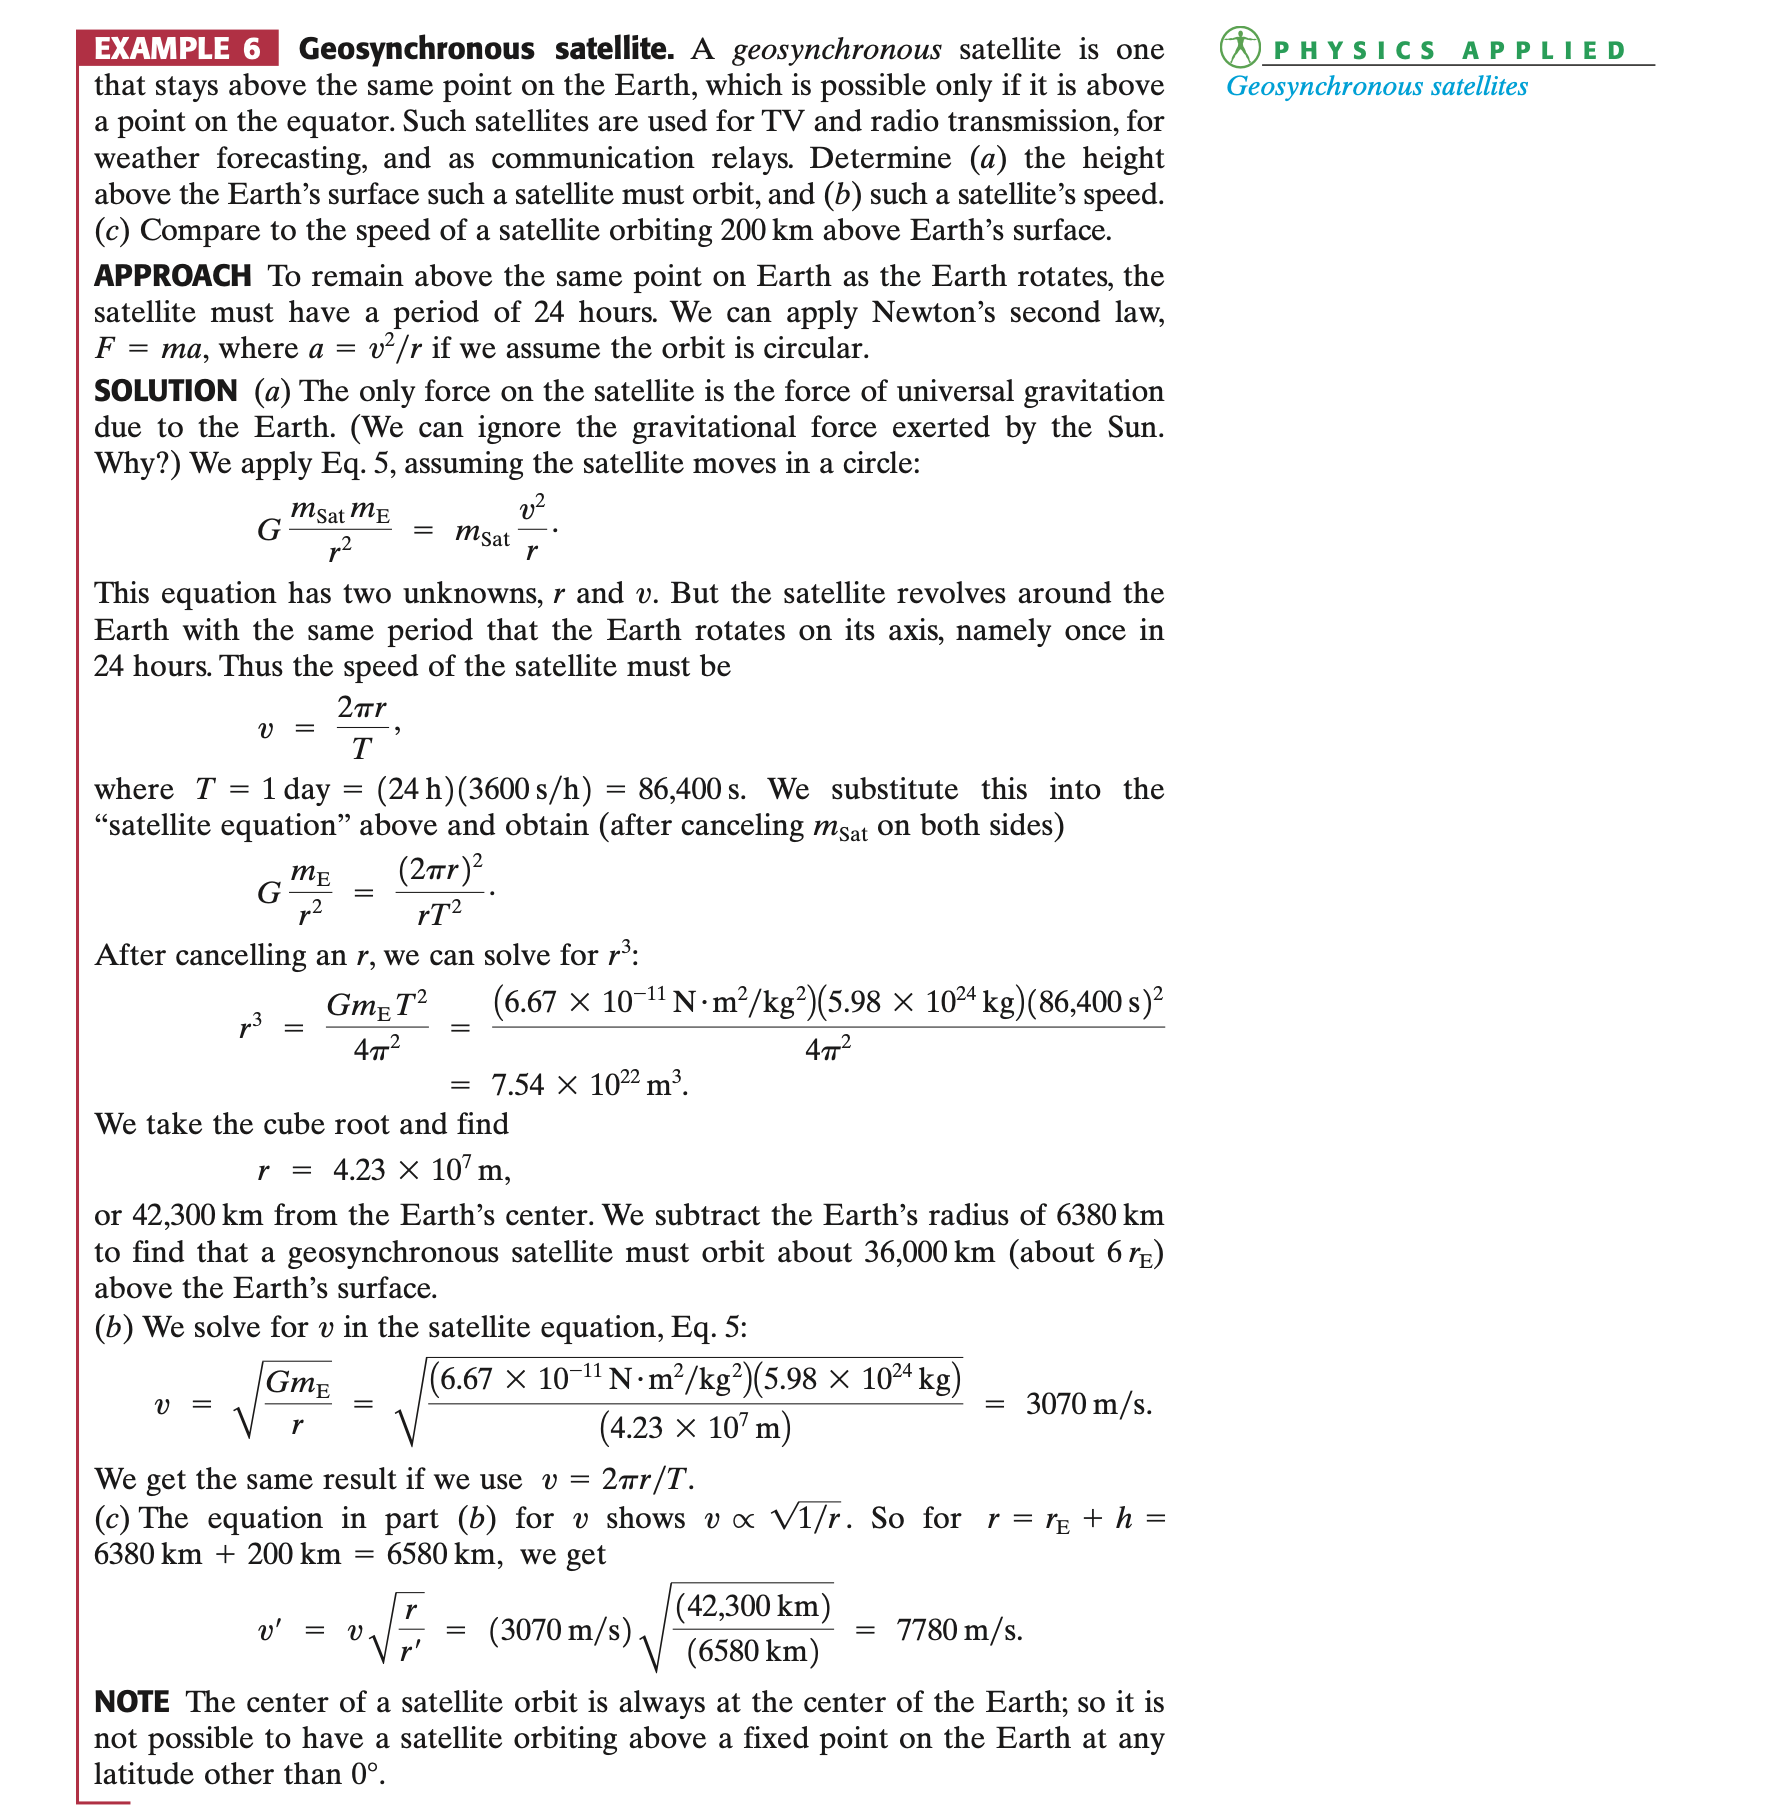
\includegraphics[scale = 0.5]{Examples/Dynamica/6.6.png}
    
% \end{ex}


\newpage

\section{Arbeid en energie}

\vspace{0.5cm}

\begin{theo}[Arbeid en energie]{Arbeid en energie}

    Arbeid is een scalaire grootheid voor energietransfer, andersom is energie dan een scalaire grootheid voor de capaciteit om arbeid te leveren.

    \begin{itemize}
    
        \item{Arbeid en energie door een constante kracht}
        
            De arbeid geleverd door een constante kracht is gelijk aan de volgende formule:
            \begin{equation*}
                W = F_{||}d = Fdcos(\theta) = \Vec{F} \cdot \Vec{d}
            \end{equation*}
            \begin{center}
                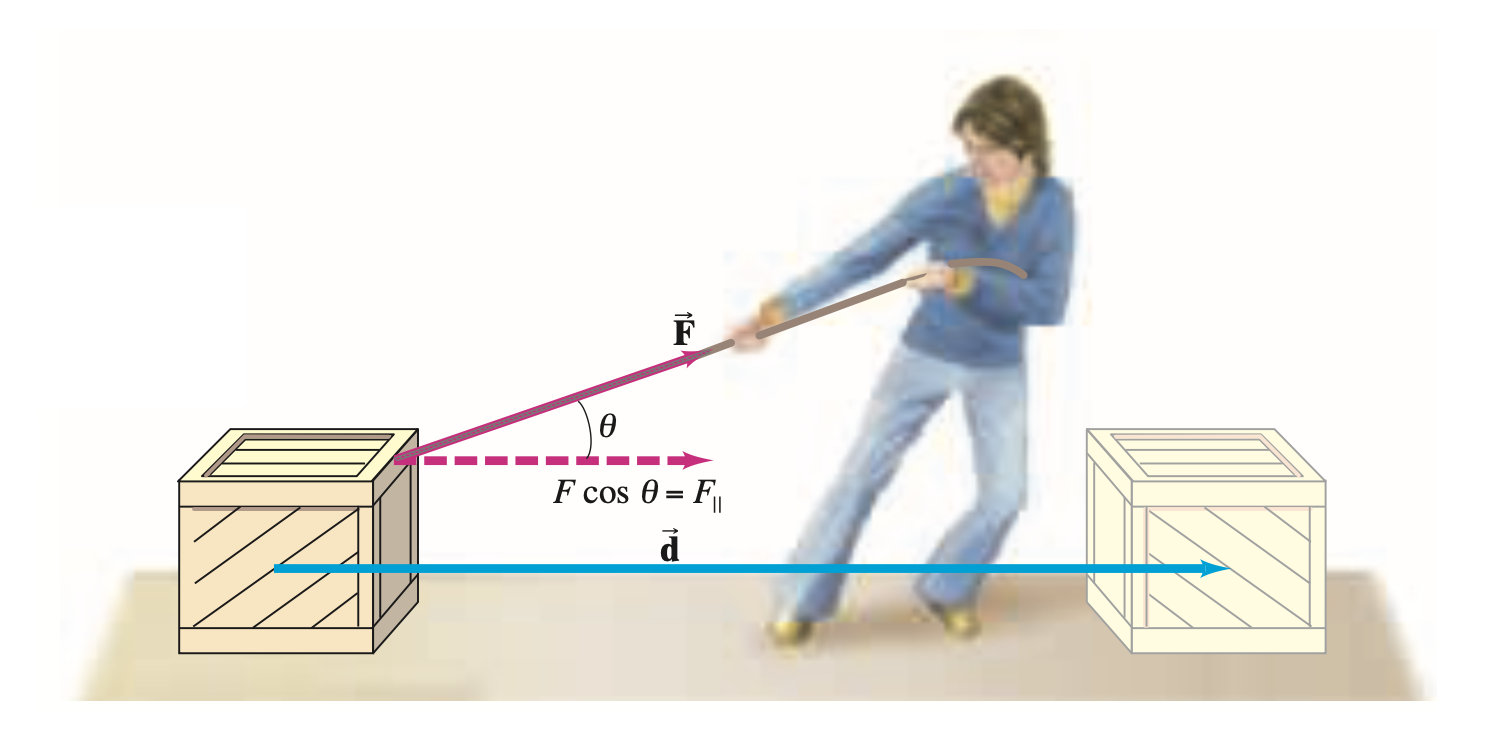
\includegraphics[scale = 0.15]{Images/Dynamica/Arbeid bij constante kracht.png}
            \end{center}
        \item{Arbeid en energie door een variabele kracht}
        
            Stel het voorwerp wordt bewogen door een variabele kracht over een pad $ a \to b $. We kunnen dit pad opsplitsen in infinitesimalen delen $ d\Vec{\ell} $. Als we nu integreren over het pad, dan krijgen we: 
            \begin{equation*}
                W = \int_{a}^{b}  F_{||}d\ell = \int_{a}^{b} F \cos\theta d\ell = \int_{a}^{b} \Vec{F} \cdot d\Vec{\ell}
            \end{equation*}
    \end{itemize}
\end{theo}

\begin{app}[Terugroepkracht van schroefveren]{Terugroepkracht van schroefveren}
    
    \begin{minipage}{.68\textwidth}
    
    Het uittrekken of samendrukken van een veer veroorzaakt een kracht, namelijk de terugroepkracht: 
    
    \begin{equation*}
        \Vec{F}_s = -k\Vec{x}
    \end{equation*}
    
    De arbeid geleverd door de veer hangt kunnen we ook berekenen:
    
    \begin{equation*}
        W_s = \int_0^x \Vec{F}_s \cdot d\Vec{x} = -\dfrac{1}{2}kx^2
    \end{equation*}

    Deze zal gelijk zijn bij samendrukken en uitrekken. \\

    \textbf{Opmerking}: de formule is geldig als de massa begint in de oorsprong en samengedrukt/uitgerokken wordt tot een punt x
    
    % Hieruit volgt dus ook dat $ W_{net} = 0 $ als we van $ -x \to x $, want:
    
    % \begin{equation*}
    %     W_{net} = W_{s,uit} + W_{s,sam} = -\dfrac{1}{2}kx^2 + \dfrac{1}{2}kx^2 = 0
    % \end{equation*}
    
    \end{minipage} 
    \begin{minipage}{.32\textwidth}
    
        \centering
        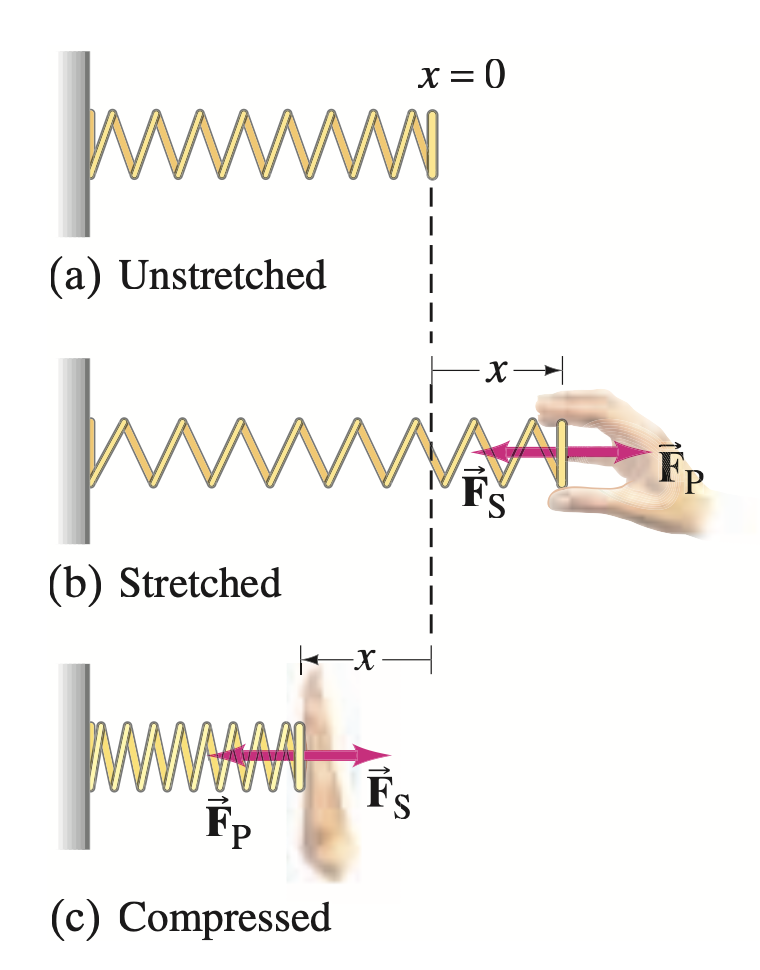
\includegraphics[scale = 0.325]{Images/Dynamica/Schroefveer.png}
        
    \end{minipage}
\end{app}

\begin{lem}[Arbeid - Kinetische energie theorema]{Arbeid Kinetische energie theorema}

De netto-arbeid $ W_{\text{net}} $ geleverd door een voorwerp wordt bepaald door de netto-kracht $ F_{\text{net}} $. Stel we hebben een variabele (of een constante) kracht die inoefent op een voorwerp, we berekenen nu de netto-arbeid:

\vspace{-0.6cm}
\begin{align*}
    W_{\text{net}} &= \int_i^f \Vec{F}_{\text{net}} \cdot d\Vec{\ell} \\
            &= \int_i^f F_{||}d\ell \\
        %    \intertext{We weten dat de parallelle versnelling gelijk is aan de verandering in de snelheid, dus:}
            &= \int_i^f m\dfrac{dv}{dt}d\ell \\
            &= \int_i^f mvdv  \\
            &= \dfrac{1}{2}mv_f^2 - \dfrac{1}{2}mv_i^2 \\
            %  \quad \quad (F_{\text{net}} = ma, \ a = \dfrac{v_2^2 - v_1^2}{2d}) \\ 
            &= \Delta K 
\end{align*}

\noindent Wat we hierboven bewezen hebben is het \textbf{Arbeid - Kinetische energie theorema}, in woorden: 

\vspace{0.3cm} \noindent  `Wanneer de enige verandering in het systeem de snelheid is, dan is de arbeid verricht door de nettokracht gelijk aan de verandering in kinetische energie van het systeem.`

\end{lem}


\newpage

\section{Behoud van energie}

\vspace{0.5cm}

\begin{theo}[Conservatieve en niet-conservatieve krachten]{Conservatieve en niet-conservatieve krachten}
    Een \textbf{conservatieve kracht} is een kracht waarbij de netto-arbeid geleverd door deze kracht nul is bij een gesloten baan, onafhankelijk is van de afgelegde weg. Bijvoorbeeld: 
    \begin{itemize}
        \item de gravitatiekracht: $ \Vec{F}_g = m\Vec{g} $      
        % \\
        % \begin{minipage}{.48\textwidth}
        %     \vspace*{\fill}
        %     \begin{align*}
        %         W &= -\int_a^b mg\hat{k}d\Vec{r} \\
        %           &= -mg\int_a^b\hat{k}(dx\hat{i}+dy\hat{j}+dz\hat{k}) \\
        %           &= -mg\int_a^bdz \\
        %           &= -mg(z_b - z_a)
        %     \end{align*}
        %     \vspace*{\fill}
            
        % \end{minipage} 
        % \begin{minipage}{.25\textwidth}
        
        %     \centering
        %     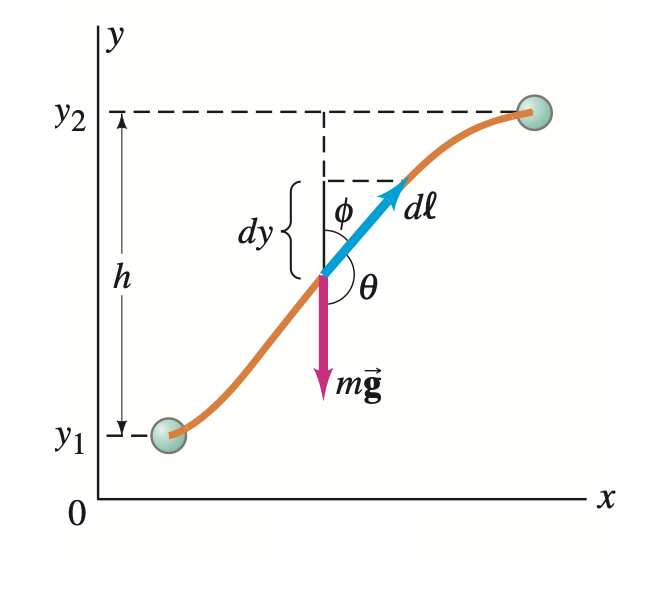
\includegraphics[scale = 0.225]{Images/Dynamica/ConservatieveZwaartekracht.png}
            
        % \end{minipage}
        \item de veerkracht: $ \Vec{F}_s = -k\Vec{x} $
    \end{itemize}
    
    \noindent Een \textbf{niet-conservatieve kracht} is een kracht waarbij de netto-arbeid geleverd door deze kracht afhankelijk is van de gevolgde weg 
    % \\ \\
    % \begin{minipage}{.44 \textwidth}
    %         \noindent\fbox{\parbox{\textwidth}{
    %         A crate is pushed slowly at constant speed across a rough floor
    %         from position 1 to position 2 via two paths: one straight and one curved. The pushing force $ F_P $ is in the direction of motion at each point. (The friction force opposes the motion.) Hence for a constant magnitude pushing force, the work it does is $ W = F_Pd$ , so if $ d $ is greater (as for the curved path), then $ W $  is greater. The work done does not depend only on points 1 and 2; it also depends on the path taken.}}       
    % \end{minipage} 
    % \begin{minipage}{.54\textwidth}
    %     \centering
    %     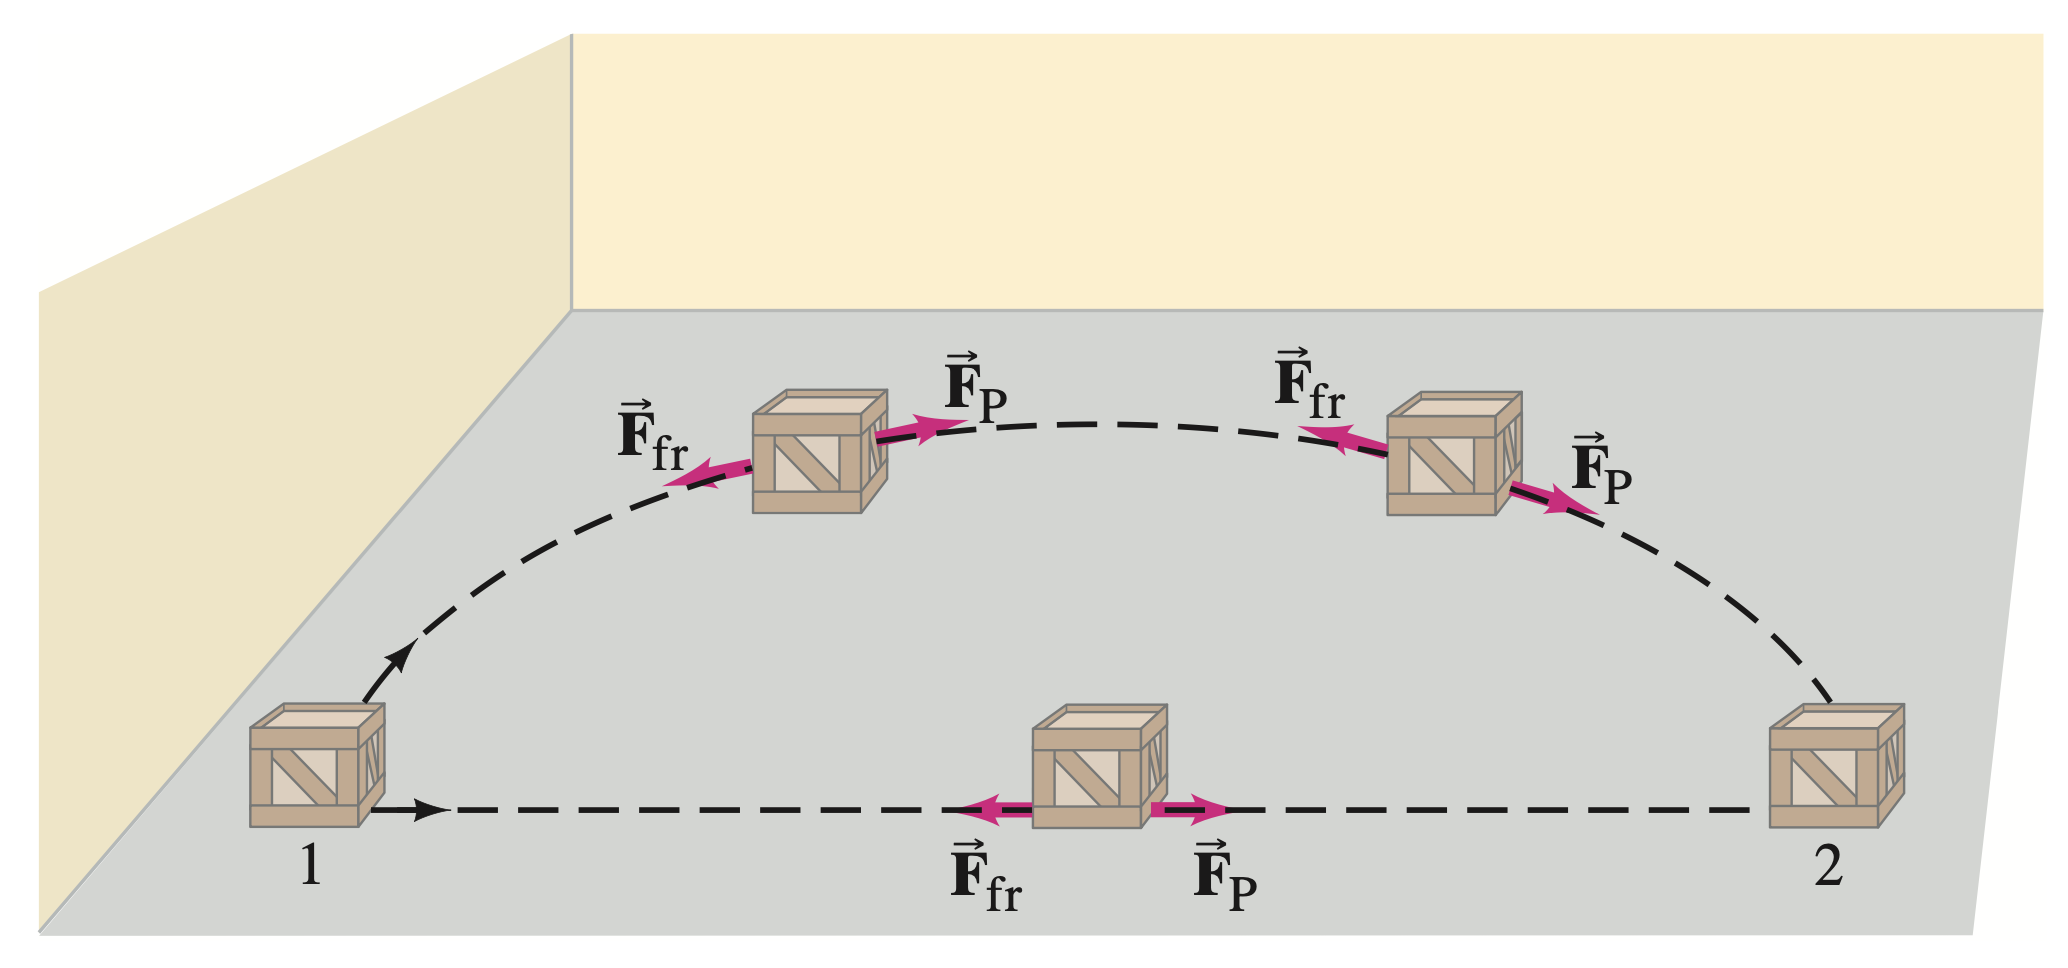
\includegraphics[scale = 0.2]{Images/Dynamica/NietConservatief.png}
    % \end{minipage}
\end{theo}

% \begin{theo}[Niet-conservatieve kracht]{Niet-conservatieve kracht}
%     Een \textbf{niet-conservatieve kracht} is een kracht waarbij de netto-arbeid geleverd door deze kracht afhankelijk is van de gevolgde weg \\ \\
%         \begin{minipage}{.44 \textwidth}
%                 \noindent\fbox{\parbox{\textwidth}{
%                 A crate is pushed slowly at constant speed across a rough floor
%                 from position 1 to position 2 via two paths: one straight and one curved. The pushing force $ F_P $ is in the direction of motion at each point. (The friction force opposes the motion.) Hence for a constant magnitude pushing force, the work it does is $ W = F_Pd$ , so if $ d $ is greater (as for the curved path), then $ W $  is greater. The work done does not depend only on points 1 and 2; it also depends on the path taken.}}       
%         \end{minipage} 
%         \begin{minipage}{.54\textwidth}
%             \centering
%             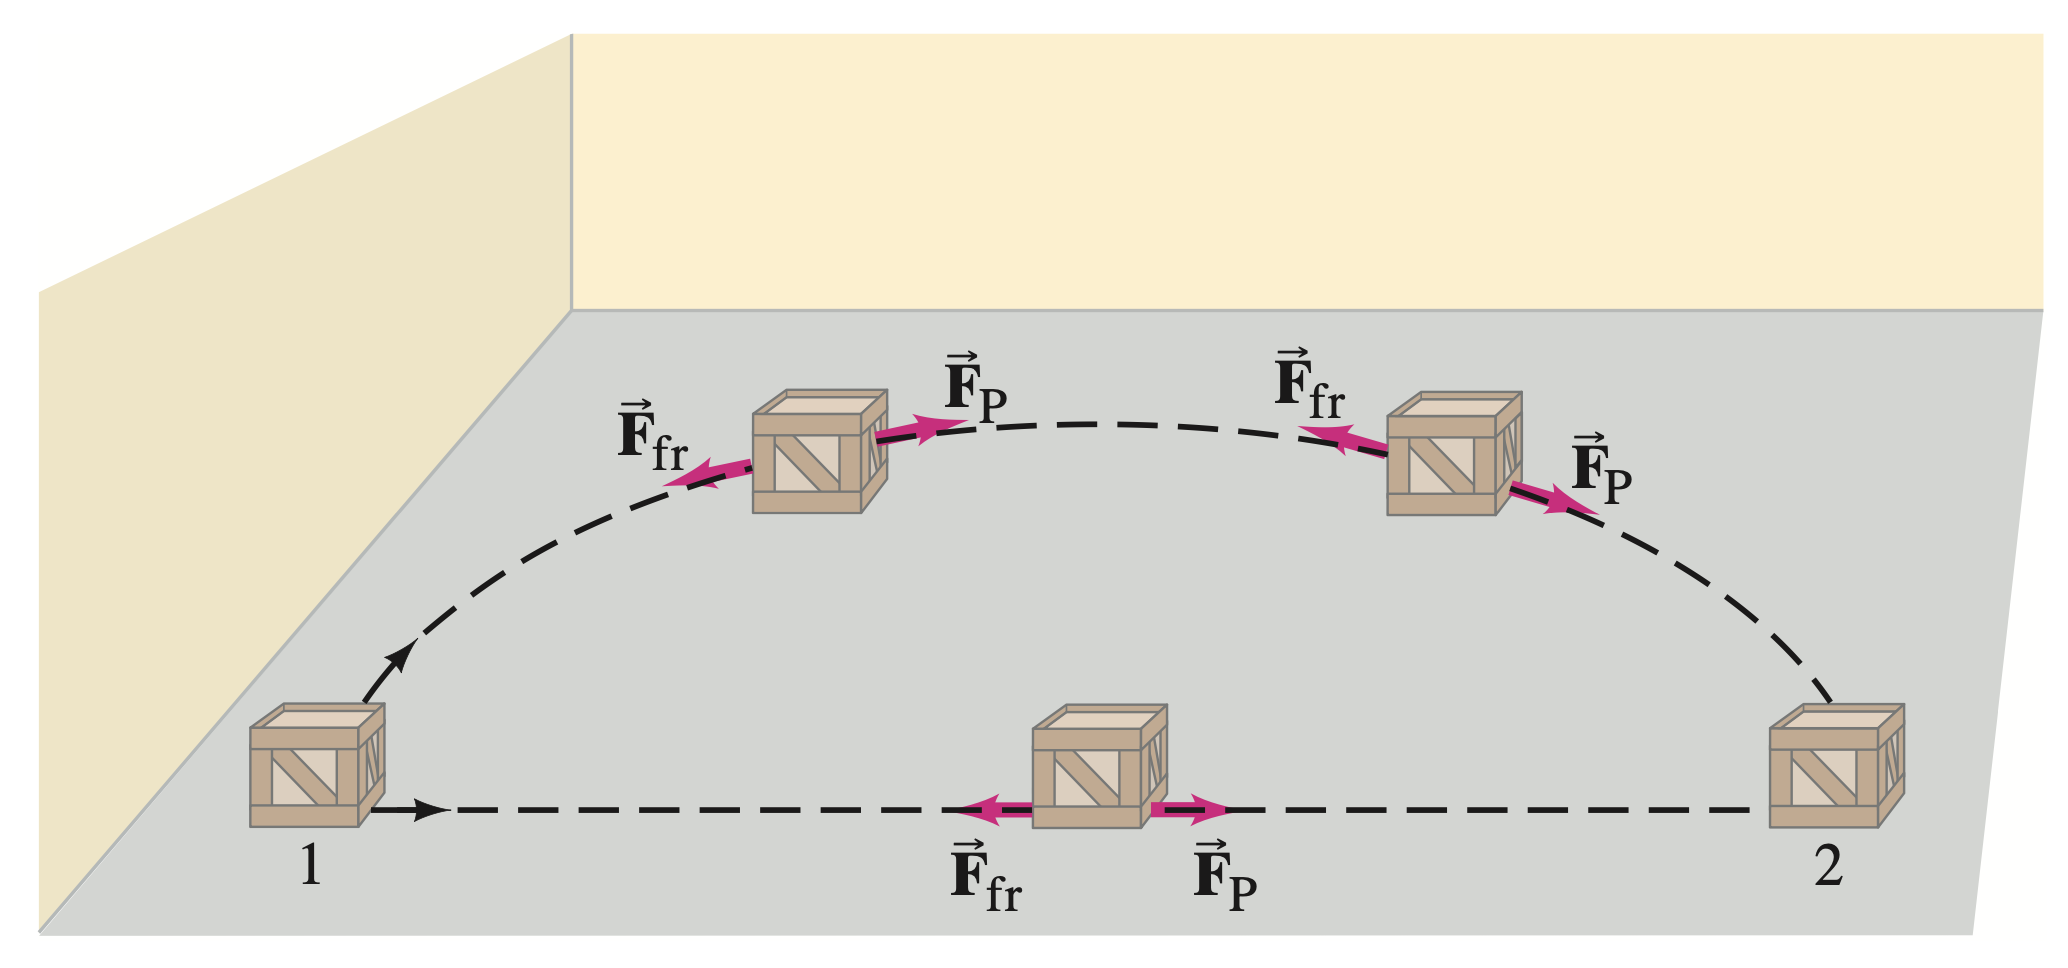
\includegraphics[scale = 0.2]{Images/Dynamica/NietConservatief.png}
%         \end{minipage}
% \end{theo}

\begin{theo}[Potentiële energie]{Potentiële energie}
    
    % Vanaf dit deelhoofdstuk spreken we ook van \textbf{potentiele energie} $ U $, wat geassocieerd wordt met krachten die afhangen van positie of afhangen van omgeving, dus: conservatieve krachten. \\
    
    \noindent De arbeid geleverd door een conservatieve kracht is gelijk aan het tegengestelde van de verandering in potentiële energie: 
        \begin{equation*}
            \Delta U = U_2 - U_1 = \int_1^2dU = -\int_1^2 \Vec{F}\cdot d\Vec{r} = -W
        \end{equation*}
    
    \noindent Het is belangrijk om aan te halen dat het \textbf{verschil} in potentiële energie onafhankelijk is van het referentiestelsel. Hierdoor kunnen we de volgende redenering maken:
    \begin{align*}
        \hspace{4.5cm} U(\Vec{r}) - U(\Vec{r}_1) &=  -\int_{\Vec{r}_1}^{\Vec{r}} \Vec{F}\cdot d\Vec{r} \quad \quad (meestal \ kiezen \ we \  U_1 = 0) \\
            -dU &= \Vec{F}\cdot d\Vec{r}  \\
                % &= F_Tdr \\
                &= drFcos(\theta) 
    \end{align*}
    Uit deze berekeningen kunnen we een belangrijke formule halen:
    \begin{equation*}
        F_T = Fcos(\theta) = -\dfrac{dU}{dr}
    \end{equation*}
    We kunnen deze vondst veralgemenen naar de 3 dimensies:
    \begin{equation*}
        \Vec{F} = -\nabla U = -\tfrac{\theta}{\theta x}U\hat{i} - \tfrac{\theta}{\theta y}U\hat{j} - \tfrac{\theta}{\theta z}U\hat{k}
    \end{equation*}
    
\end{theo}

\begin{lem}[Behoud van energie]{Bbehoud van energie}

    De wet van behoud van energie stelt dat energie niet kan worden gecreëerd of vernietigd - alleen omgezet van de ene vorm van energie in een andere. In formulevorm:
    
    \begin{equation*}
        \Delta K + \Delta U = W_{nc} 
    \end{equation*}
    \vspace{-0.5cm}
\end{lem}

\newpage

\begin{lem}[Behoud van mechanische energie]{Behoud van mechanische energie}
    We bundelen even wat vondsten van hiervoor samen:
    \begin{align*}
        K_b - K_a &= -(U_b - U_a) = U_a - U_b \\
        K_a + U_a &= K_b + U_b \\ 
        E_a = (K + U)_a &= (K + U)_b = E_b
    \end{align*}
    
    \noindent We zien nu dus dat de totale mechanische energie $ E = K + U $ van een deeltje constant blijft ($ E_a = E_b $) als de inwerkende krachten die arbeid leveren conservatief zijn. In formulevorm:
    
    \begin{equation*}
        \Delta E = \Delta K + \Delta U = 0
    \end{equation*}
    \vspace{-0.5cm}
\end{lem}

% \begin{app}[Arbeid geleverd door een veer]{Arbeid geleverd door een veer}

%     We berekenen het verschil in potentiele energie van $ 0 \to x $ met x positief of negatief:
    
%     \begin{align*}
%         \Delta U = U(x) - U(0) = -\int_0^x (-kx)dx = \dfrac{1}{2}kx^2 = - W_s
%     \end{align*}
    
%     \noindent De mechanische energie blijft constant als de inwerkende krachten conservatief zijn, wat natuurlijk zo is bij een veer. We bekomen de volgende formule indien we zeggen dat $ U = U(x) $:
    
%     \begin{equation*}
%         \dfrac{1}{2}mv^2_1 + \dfrac{1}{2}kx^2_1 = \dfrac{1}{2}mv^2_2  + \dfrac{1}{2}kx^2_2
%     \end{equation*}
% \end{app}

\begin{theo}[Vermogen]{Vermogen}
    Het \textbf{vermogen} is een scalaire grootheid voor arbeid per tijdseenheid, uitgedrukt in Watt.
    \begin{itemize}
        \item \textbf{Gemiddelde:} $ P_{gem} = \dfrac{W}{\Delta t} $ 
        \item \textbf{Ogenblikkelijke:} $ P = \dfrac{dW}{dt} = \dfrac{dE}{dt} $, want arbeid = energie transformatie! \\
        We krijgen uit de definitie van arbeid: $ P = \Vec{F} \cdot \dfrac{d\Vec{r}}{dt} = \Vec{F} \cdot \Vec{v} $
    \end{itemize}
\end{theo}

\newpage

\section{Impuls}

\vspace{0.5cm}

\begin{theo}[Impuls]{Impuls}
    Impuls is een vectoriële grootheid die de hoeveelheid van beweging weergeeft. In formulevorm: 
        \begin{equation*}
            \Vec{p} = m\Vec{v}.
        \end{equation*}
        
    \noindent Met dit nieuw begrip kunnen we de tweede wet van Newton herdefiniëren:
    \begin{equation*}
        \sum \Vec{F} = m\Vec{a} = \dfrac{d(m\Vec{v})}{dt} = \dfrac{d\Vec{p}}{dt}.
    \end{equation*}

    \vspace{-0.3cm}

    % \noindent \textbf{Opmerking:} Om het impuls van een voorwerp te veranderen is een kracht nodig!
\end{theo}

\begin{lem}[Behoud van impuls]{Behoud van impuls}
    De wet van de behoud van impuls stelt dat de \textbf{totale impuls} $ \Vec{P} $ van een geïsoleerd stelsel van deeltjes constant is wanneer: 
    \begin{equation*}
         \sum \Vec{F}_{ext} = \dfrac{\sum_i d\Vec{p}_i}{dt} = \dfrac{d\Vec{P}}{dt} = 0.
    \end{equation*} 
    % \noindent \textbf{Dus:} De verandering van impuls is gelijk aan de \textbf{netto}kracht op het systeem.
\end{lem}

\begin{app}[Elastische botsing]{Elastische botsing}

    Bij een elastische botsing wordt de kinetische energie behouden. We kunnen nu met deze wet en de wet van behoud van impuls te werk gaan. Enerzijds krijgen we uit de wet van behoud van impuls: 
    
    \begin{equation}
        m_av_a + m_bv_b = m_av_a' + m_bv_b'
    \end{equation}
    
    \noindent Anderzijds uit de wet van behoud van kinetische energie bij elastische botsing:
    \begin{equation}
        \dfrac{1}{2}m_av_a^2 + \dfrac{1}{2}m_bv_b^2 = \dfrac{1}{2}m_a{v_a'}^{2} + \dfrac{1}{2}m_b{v_b'}^{2}
    \end{equation}
    
    \noindent We kunnen (1) herschrijven als volgt:
    
    \begin{equation}
        m_a(v_a - v_a') = m_b(v_b' - v_b)
    \end{equation}
    
    \noindent We kunnen ook (2) herschrijven als volgt:
    
    \begin{equation}
        m_a(v_a^2 - {v_a'}^{2}) = m_b({v_b'}^{2} - v_b^2)
    \end{equation}
    
    \noindent Wegens $ (a-b)(a+b) = a^2-b^2 $ kunnen we (4) weer herschrijven:
    
    \begin{equation}
        m_a(v_a - v_a')(v_a + v_a') = m_b(v_b' - v_b)(v_b' + v_b)
    \end{equation}

    % \newpage
    
    \noindent Tenslotte kunnen we (5) delen door (3) en bekomen we:

    \vspace{-0.3cm}
    
    \begin{align*}
        v_a - v_b  &= -(v_a' - v_b') 
    \end{align*}
    
    % \noindent Dit is een interessant resultaat: het vertelt ons dat bij elke elastische head-on botsing de relatieve snelheid van de twee voorwerpen na de botsing dezelfde grootte (maar tegengestelde richting) heeft als vóór de botsing, ongeacht de massa's. 

    \vspace{-0.3cm}

\end{app}
    
\begin{app}[Inelastische botsing]{Inelastische botsing}
    
    Bij een inelastische botsing wordt de kinetische energie niet behouden. Desondanks wordt de totale energie altijd behouden en dus ook het vectoriële totale impuls. Als de botsing compleet inelastisch is (dus dat de voorwerpen één massa vormen na botsing), dan kunnen we de wet van behoud van impuls toepassen en de volgende formule krijgen:
    
    \begin{equation*}
        m_a\Vec{v}_a + m_b\Vec{v}_b = (m_a + m_b)\vec{v}
    \end{equation*}

\end{app}

% \begin{ex}[Voorbeeld: Botsingen in meerdere dimensies]{Botsingen in meerdere dimensies}
%     \centering
%     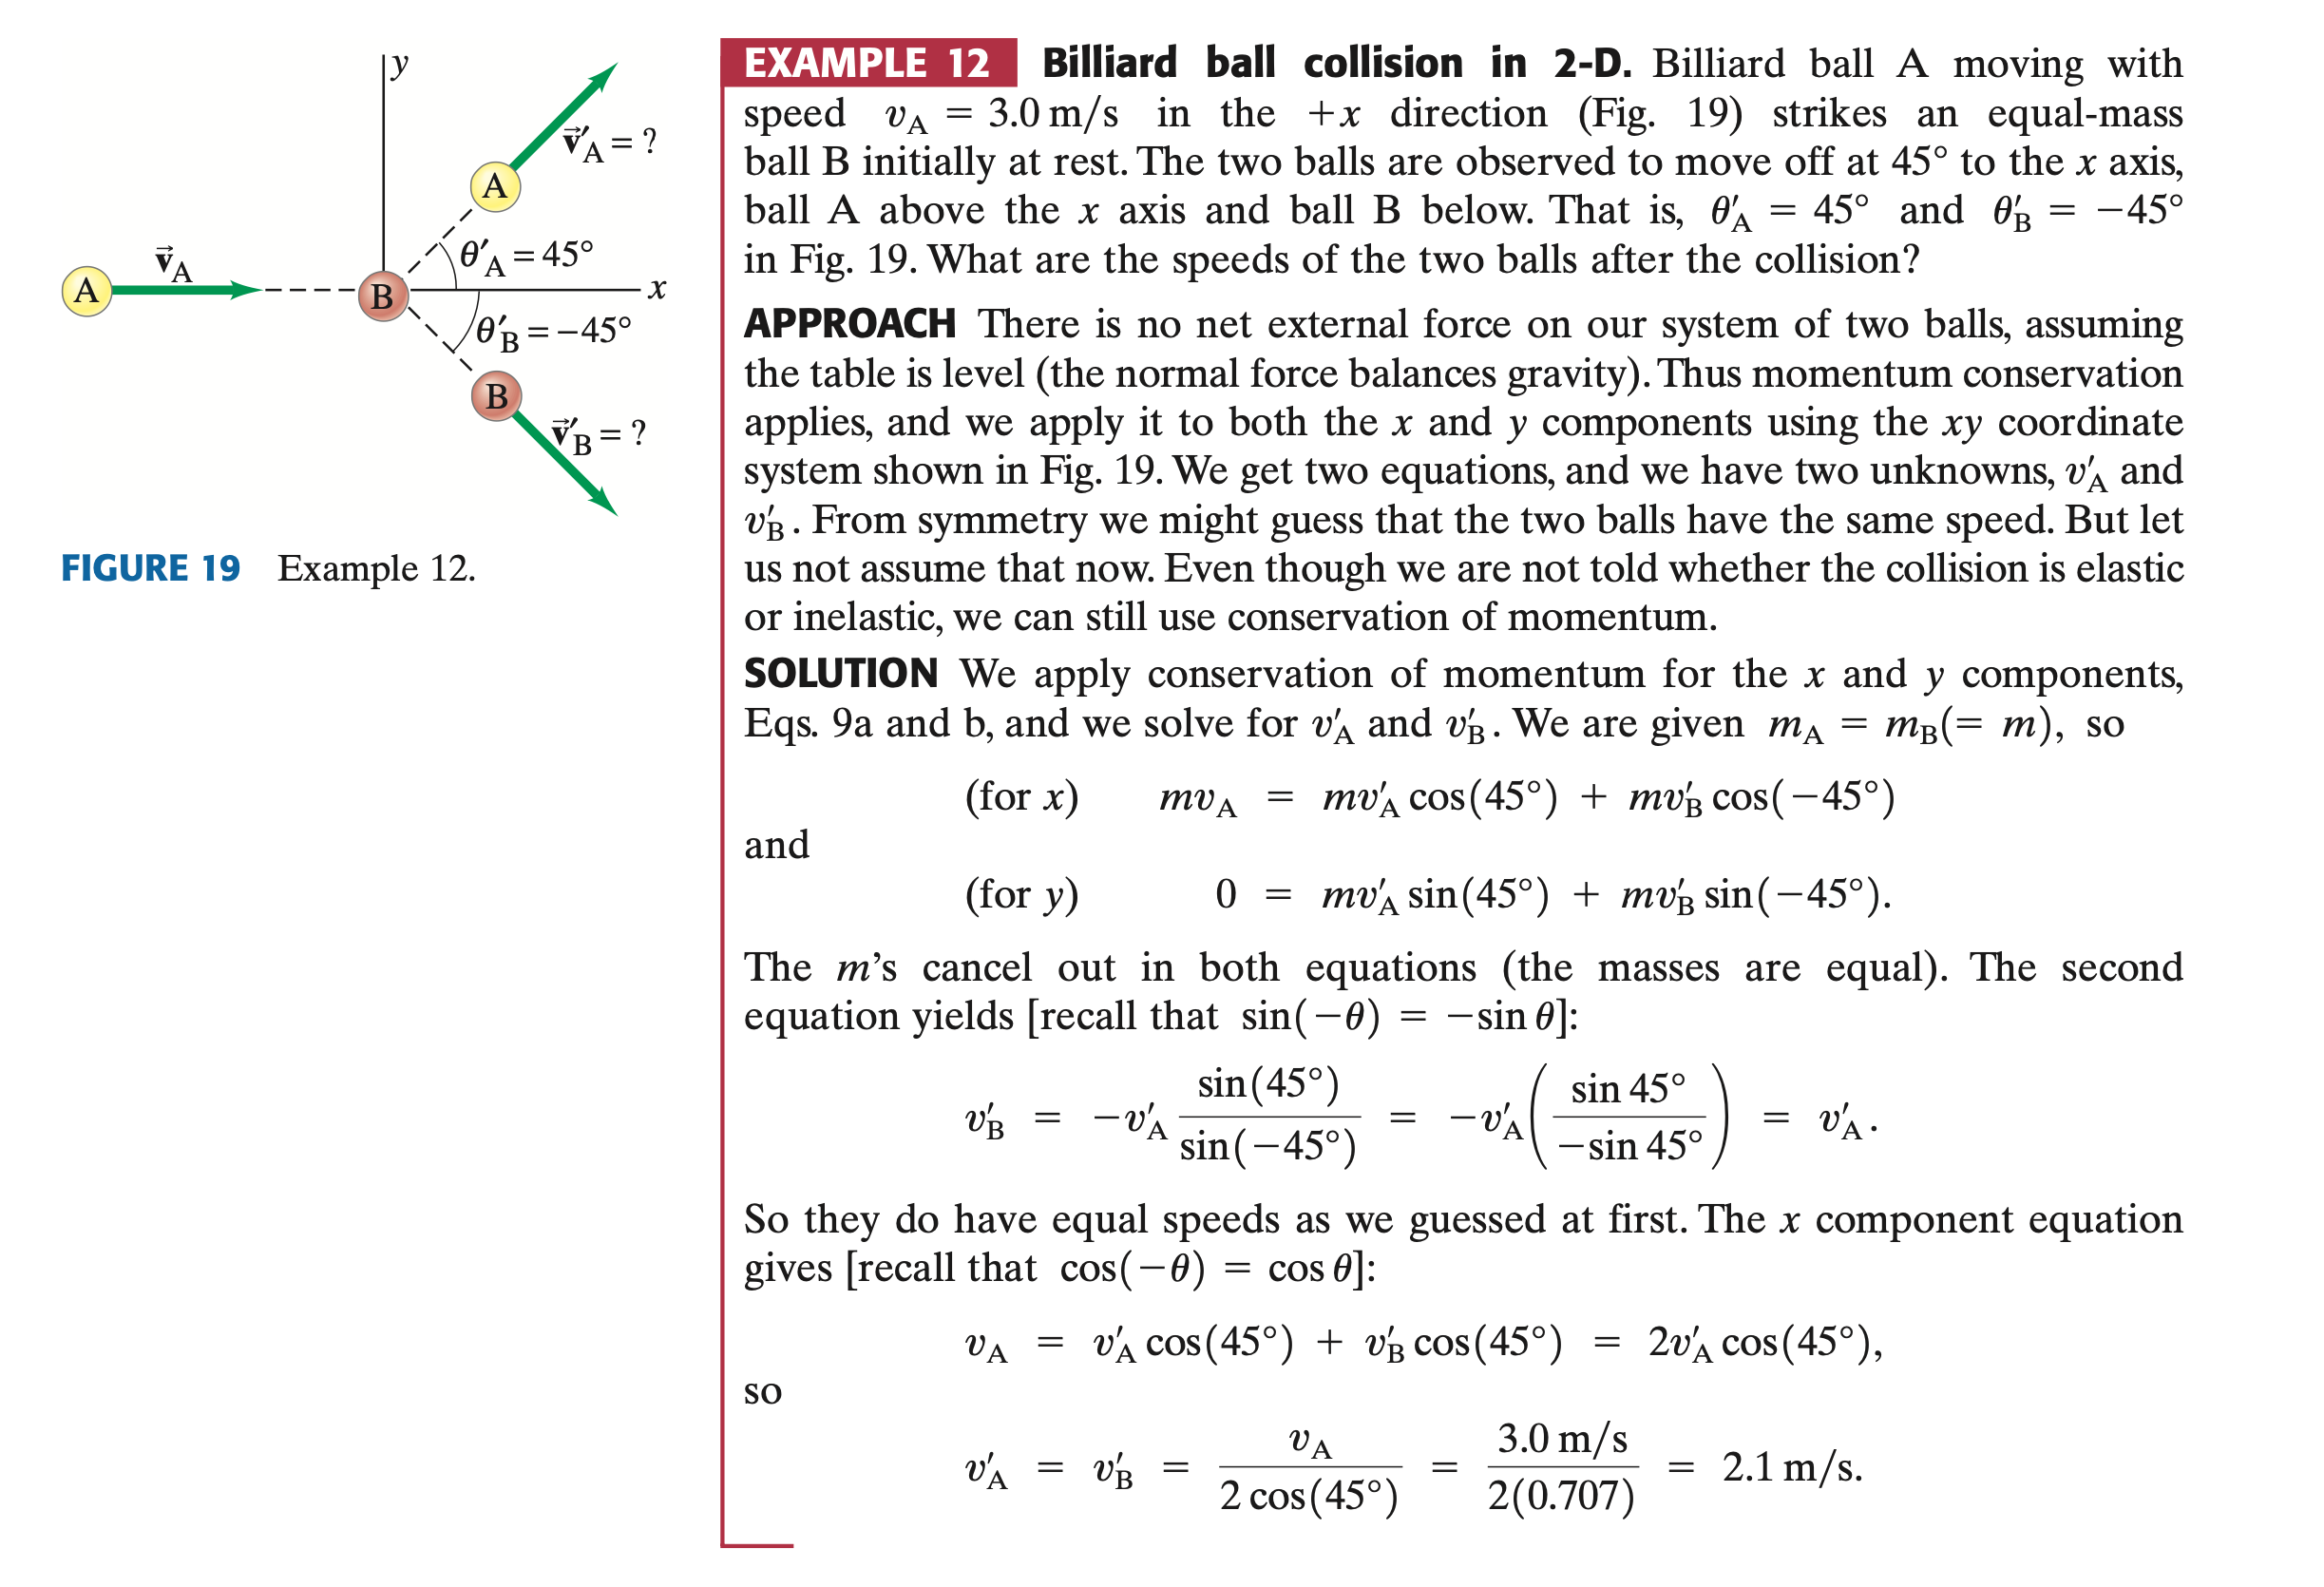
\includegraphics[scale = 0.36]{Examples/Dynamica/9.12.png}
% \end{ex}


\newpage

\section{Rotatie - Krachtmoment - Impulsmoment}

\vspace{0.5cm}

% \begin{theo}[Rotationele grootheden]{Rotationele grootheden}
%     \begin{minipage}{.56\textwidth}
%         \begin{itemize}
%             \item \textbf{Hoekverplaatsing:} $ \Delta \theta = \theta_2 - \theta_1 $
%             \item \textbf{Hoek:} $ \theta = \dfrac{\ell}{R}$  
%             \item \textbf{Hoeksnelheid:} $ (= \dfrac{\text{rad}}{s})$
%             \begin{itemize}
%                 \item \textbf{Gemiddelde:} $ \omega_{gem} = \dfrac{\Delta\theta}{\Delta t}$
%                 \item \textbf{Ogenblikkelijke:} $ \omega = \lim_{\Delta t \to 0} \dfrac{\Delta\theta}{\Delta t} = \dfrac{d\theta}{dt} $ 
%             \end{itemize}
%             \item \textbf{Hoekversnelling:} $ (= \dfrac{\text{rad}}{s^2}) $
%             \begin{itemize}
%                 \item \textbf{Gemiddelde:} $ \alpha_{gem} = \dfrac{\Delta\omega}{\Delta t}$
%                 \item \textbf{Ogenblikkelijke:} $ \alpha = \lim_{\Delta t \to 0} \dfrac{\Delta\omega}{\Delta t} = \dfrac{d\omega}{dt} $ 
%             \end{itemize}
%         \end{itemize}
%     \end{minipage} 
%     \begin{minipage}{.40\textwidth}
%         \centering
%         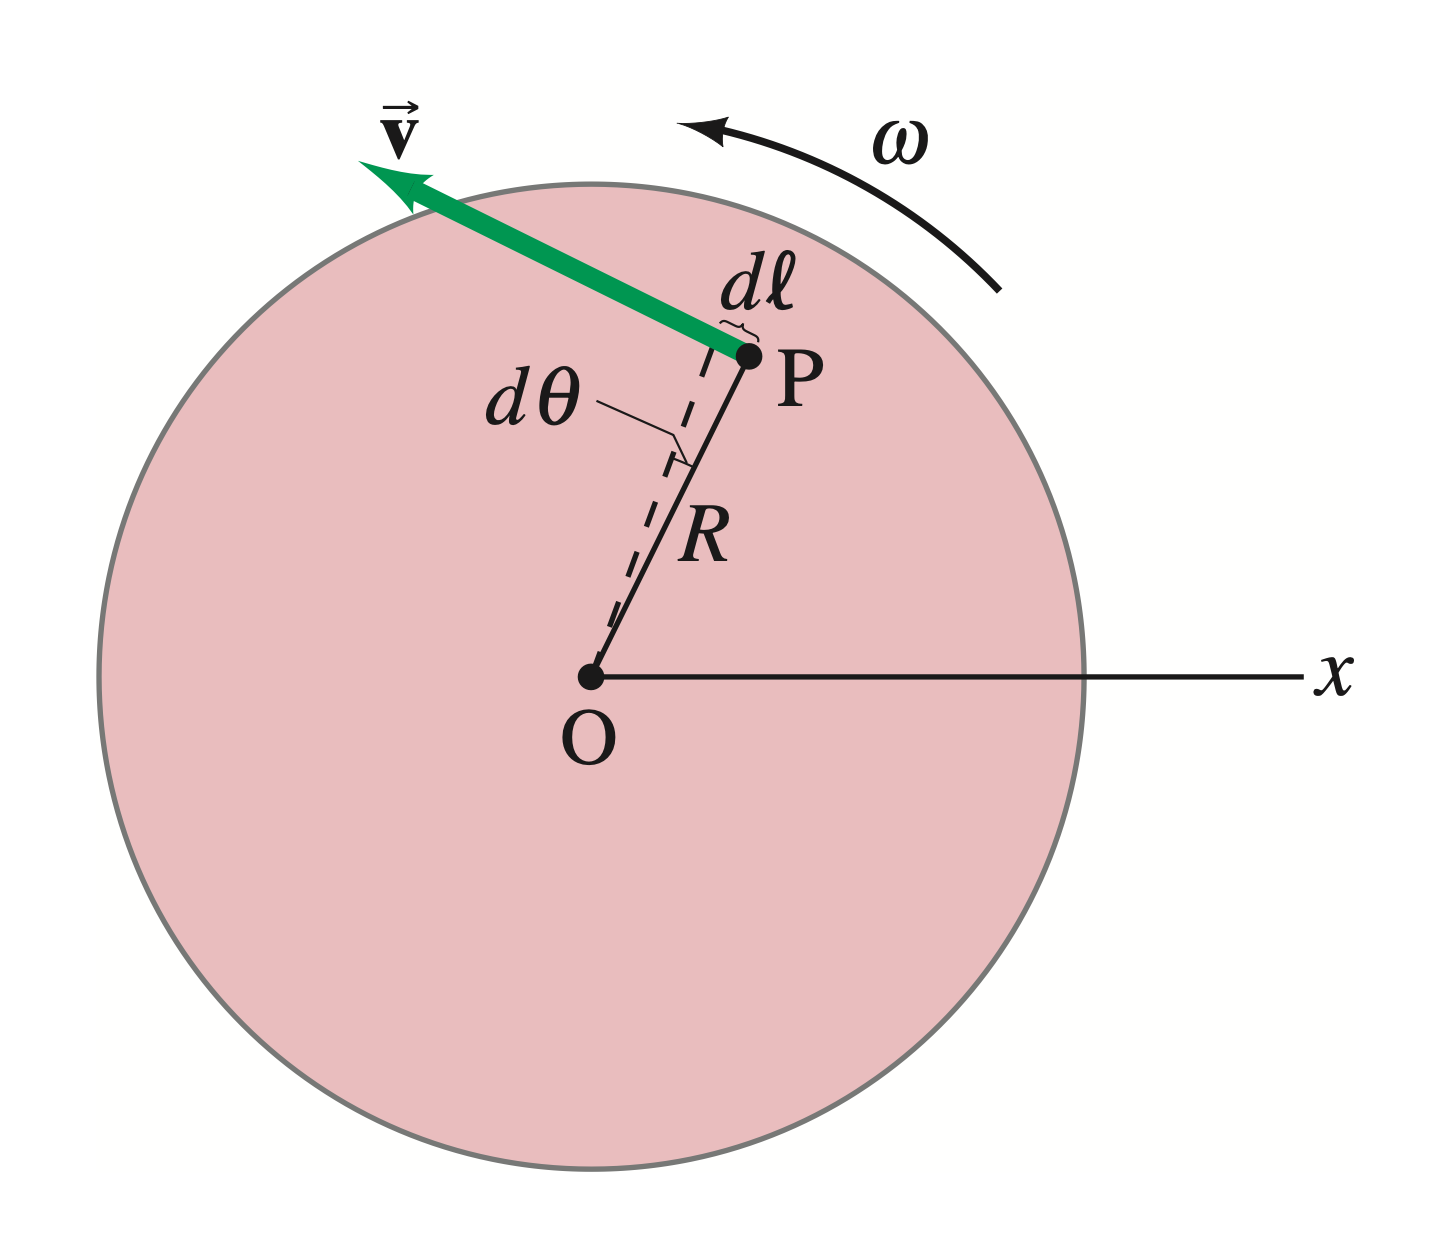
\includegraphics[scale = 0.225]{Images/Dynamica/RotatieCirkel.png}
%     \end{minipage}
% \end{theo}    

\begin{app}[Constante rotationele vs translationele versnelling]{Constante rotationele vs translationele versnelling}
    \vspace{-0.2cm}
    \begin{center}
        \def\arraystretch{2}
        \begin{tabular}{c|c}
            Rotationele beweging met constante $ \alpha $ & Translationele beweging  met constante $ a $ \\ \hline
            $ \omega = \omega_0 + \alpha t $ & $ v = v_0 +at $\\
            $ \theta = \omega_0t + \tfrac{1}{2}\alpha t^2 $ & $ x = v_0t + \tfrac{1}{2}at^2 $ \\
            $ \omega^2 = \omega_0^2 + 2\alpha\theta $ & $ v^2 = v_0^2 + 2ax $\\
            $ \omega_{gem} = \dfrac{\omega + \omega_0}{2}$ & $ v_{gem} = \dfrac{v+v_0}{2} $
        \end{tabular}
    \end{center}
\end{app}
 
\begin{theo}[Krachtmoment]{Krachtmoment}
    Het draaieffect (de hoekversnelling) van een kracht wordt bepaald door de grootte van de kracht, de richting/zin van de kracht en de "\textbf{momentarm}": afstand tussen het aangrijpingspunt van de kracht en de rotatie-as. Het \textbf{krachtmoment} is het rotationele equivalent van het translationele kracht, in formulevorm:

    \begin{equation*}
        \Vec{\tau} = \Vec{r} \times \Vec{F}
    \end{equation*}

    \noindent De grootte van het krachtmoment wordt gegeven door de volgende formule:

    \begin{equation*}
       \tau = rF\sin(\theta) = r(ma)\sin(\theta) = (m(rsin(\theta))^2)\alpha = I\alpha
    \end{equation*}

    % \noindent Sinds enkel de transversale component, de krachten, rotatie veroorzaken kunnen we de 2de wet van Newton toepassen, we vinden:

    % \begin{equation*}
    %     \tau_{net} = \sum_i \tau_i = I\alpha
    % \end{equation*}
\end{theo}

\begin{app}[Arbeid en Vermogen bij rotatie]{Arbeid en Vermogen bij rotatie}
    \begin{minipage}{.66\textwidth}
            De arbeid vericht door een object dat roteert rond een vaste as kan geschreven kan geschreven worden tegenover rotationele grootheden:
            \begin{equation*}
                W = \int \Vec{F} \cdot d\Vec{\ell} = \int F_{\perp}rd\theta
            \end{equation*}
            waarbij $ d\Vec{\ell} $ een infinitesimale afstand is loodrecht op $ r $ met grootte $ dl = rd\theta $. We weten van hierboven natuurlijk dat $ \tau = F_{\perp}r $, dus de formule wordt:
            \begin{equation*}
                W = \int_{\theta_1}^{\theta_2}\tau d\theta
            \end{equation*}
            Het vermogen bij rotatie kunnen we nu ook afleiden:
            \begin{equation*}
                P = \dfrac{dW}{dt} = \tau \dfrac{d\theta}{dt} = \tau \omega
            \end{equation*}
        \end{minipage} 
        \begin{minipage}{.33\textwidth}
            \centering
            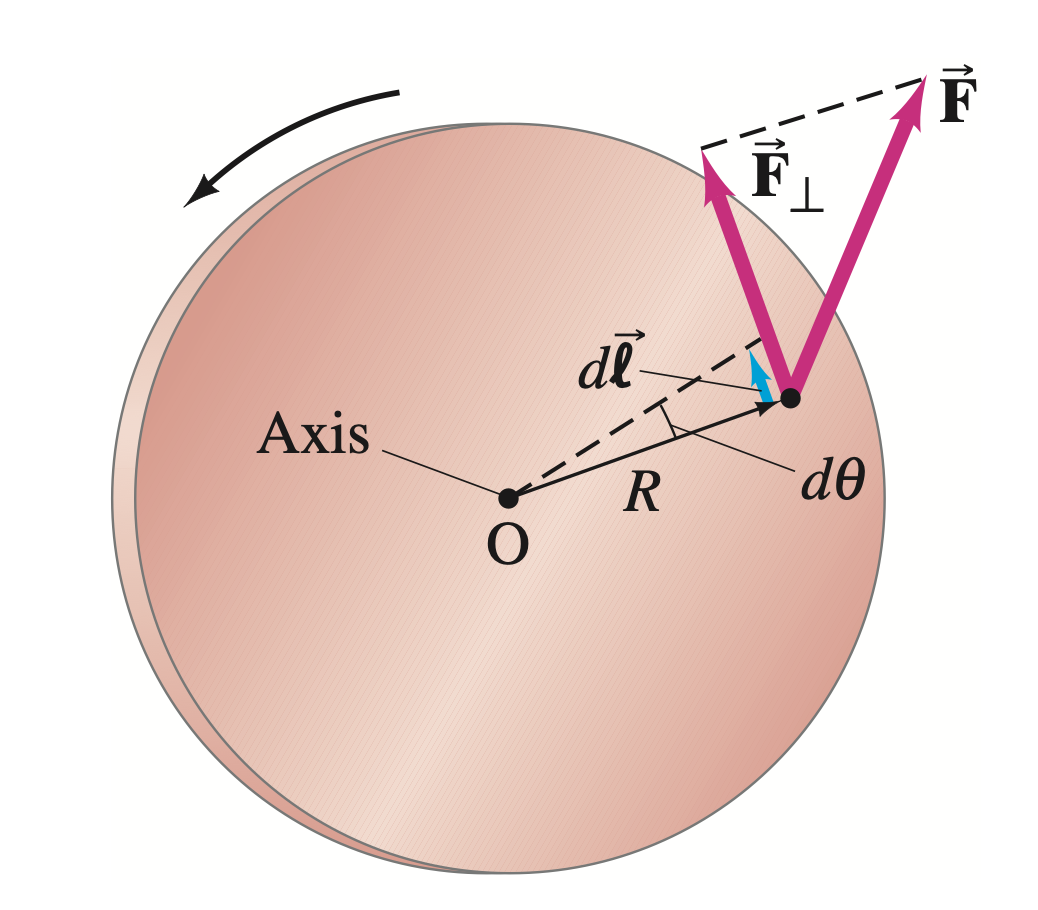
\includegraphics[scale = 0.25]{Images/Dynamica/ArbeidBijRotatie.png}
        \end{minipage}
\end{app}

\newpage

\begin{app}[Kinetische energie bij rotatie]{Kinetische energie bij rotatie}
    \vspace{-0.5cm}
    \begin{minipage}{.69\textwidth}
        Beschouw een stijf, roterend voorwerp als opgebouwd uit vele kleine deeltjes, elk met een massa $m_i$. De totale kinetische energie van het hele object is de som van de kinetische energie van alle deeltjes:
        \begin{equation*}
            K = \sum(\dfrac{1}{2}m_iv_i^2) = \sum(\dfrac{1}{2}m_ir_i^2\omega^2) =  \dfrac{1}{2}I\omega^2
        \end{equation*}
    \end{minipage} 
    \begin{minipage}{.27\textwidth}
        \centering
        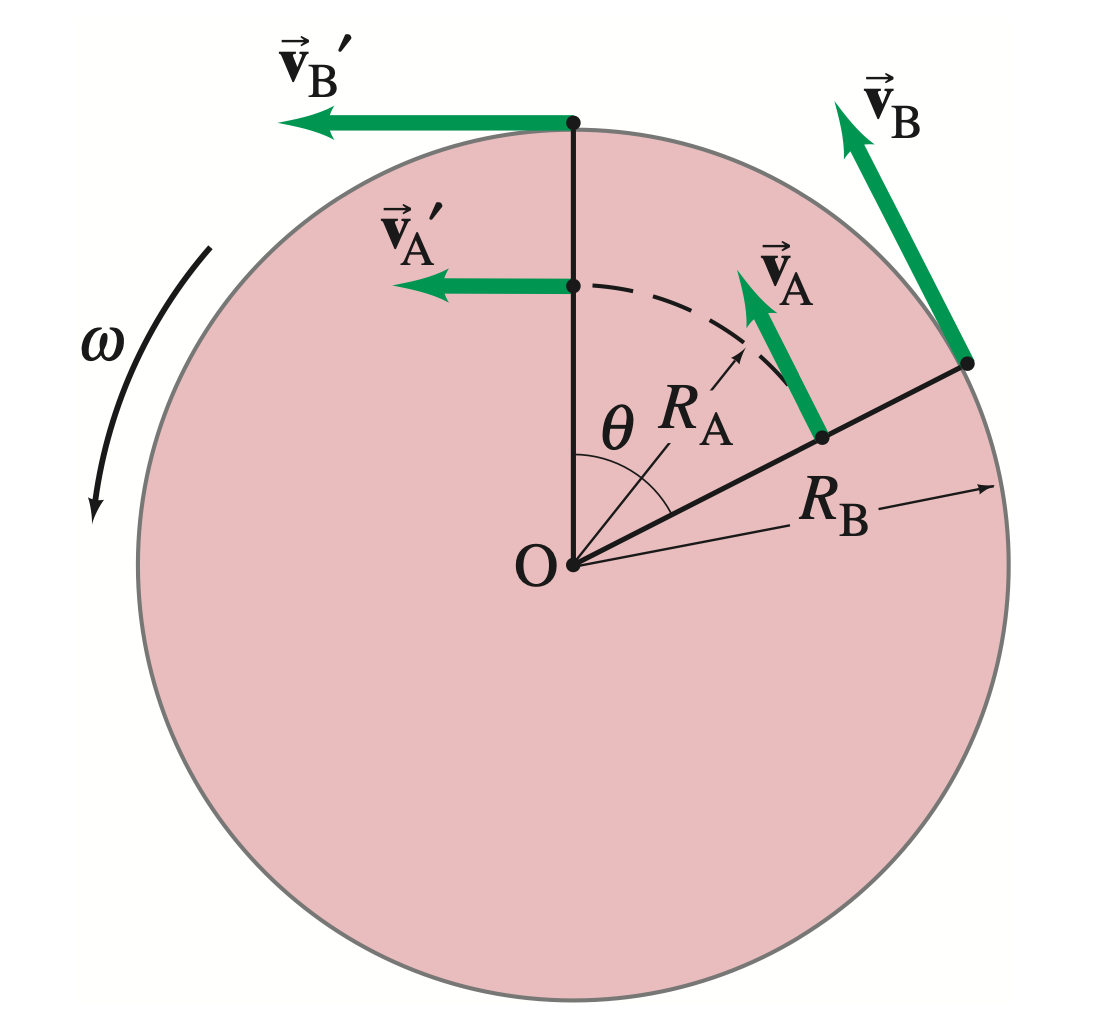
\includegraphics[scale = 0.15]{Images/Dynamica/SnelhedenOpRotatie.png}
    \end{minipage}
\end{app}

\begin{theo}[Impulsmoment]{Impulsmoment}
     Het \textbf{Impulsmoment} is de rotationele variant van het translatonele impuls, net zoals krachtmoment rotationele variant is van de translationele kracht. Het wordt gegeven door de volgende formule:
    
     \begin{equation*}
         \Vec{L} = \Vec{r} \times \Vec{p}
     \end{equation*}

     \noindent De grootte van het impulsmoment kunnen we als volgt berekenen:
     \begin{equation*}
         L = prsin(\theta) = mvrsin(\theta) = (m(rsin(\theta))^2)\omega = I\omega
     \end{equation*}
     \vspace{-0.5cm}
\end{theo}

\begin{lem}[Behoud van impulsmoment]{Behoud van impulsmoment}
    De wet van de behoud van impulsmoment stelt dat de \textbf{totale impulsmoment} ($ \Vec{L}_{net} $) van een geïsoleerd stelsel van deeltjes constant is wanneer: 
    \begin{equation*}
         \tau_{net} = \sum \tau_{ext} = \sum \dfrac{I\omega}{dt} = \dfrac{dL_{net}}{dt} = 0
    \end{equation*} 
    \vspace{-0.5cm}
\end{lem}

\begin{app}[Vergelijking: impuls – impulsmoment]{Vergelijking: impuls – impulsmoment}
    \begin{minipage}{.48\textwidth}
        \begin{center}
            
            \underline{Algemeen}: \\
            \vspace{0.25cm}
            \def\arraystretch{2.5}
            \begin{tabular}{c|c}
                impuls & impulsmoment \\ \hline
                $ \Vec{p} $ & $ \Vec{L} = \Vec{r} \times \Vec{p} $ \\ 
                $ \Vec{F} = \dfrac{d\Vec{p}}{dt} $ &  $ \Vec{\tau} = \dfrac{d\Vec{L}}{dt} $
            \end{tabular}
    
        \end{center}
    \end{minipage} 
    \begin{minipage}{.48\textwidth}
        \begin{center}
                
            \underline{Enkel bij een geïsoleerd systeem}: \\
            \vspace{0.25cm}
            \def\arraystretch{2.5}
            \begin{tabular}{c|c}
                impuls & impulsmoment \\ \hline
                behoud van impuls & behoud van impulsmoment \\ 
                $ F_{net} = \sum F_{ext} = 0 $ & $ \tau_{net} = \sum \tau_{ext} = 0 $
            \end{tabular}
        
        \end{center}
    \end{minipage}
\end{app}

% \begin{app}[Verband tussen impulsmoment en krachtmoment]{Verband tussen impulsmoment en krachtmoment}

%     Net zoals kracht zorgt voor de verandering van impuls van een voorwerp, zorgt krachtmoment voor de verandering van impulsmoment van een voorwerp: dit is het voornaamste verband.
    
%     Als we de tweede wet van newton bekijken bij rotatie, dan krijgen we de volgende formule die het verband aantoont:
    
%     \begin{equation*}
%         \sum \Vec{\tau} = I\Vec{\alpha} = I(\dfrac{d\Vec{\omega}}{dt}) = \dfrac{d(I\Vec{\omega})}{dt} = \dfrac{d\Vec{L}}{dt}
%     \end{equation*}

%     \noindent Omgekeerd kan ook als we een \textbf{puntmassa} bekijken:
%     \begin{equation*}
%         \dfrac{d\Vec{L}}{dt} = \dfrac{d(\Vec{r} \times \Vec{p})}{dt} = \dfrac{d\Vec{r}}{dt} \times \Vec{p} + \Vec{r} \times \dfrac{d\Vec{p}}{dt} = \Vec{v} \times \Vec{p} + \Vec{r} \times \Vec{F}
%     \end{equation*}
%     \noindent Het eerste lid van de som, namelijk $ \Vec{v} \times \Vec{p} $, wordt simpelweg 0, want $ \Vec{p} = m\Vec{v} $ is een lineaire combinatie van $ \Vec{v} $. Nu hebben we:
%     \begin{equation*}
%         \dfrac{d\Vec{L}}{dt} = \Vec{r} \times \Vec{F} = \tau \Rightarrow \dfrac{d\Vec{L}_{net}}{dt} = \Vec{r} \times \sum \Vec{F} = \sum \tau
%     \end{equation*}
%     % \noindent Als we nu $ \sum \Vec{F} $ pakken als de netto kracht, dan is bij een inertiaalreferentiestelsel:
%     % \begin{equation*}
%     %    \dfrac{d\Vec{L}}{dt} = \Vec{r} \times \sum \Vec{F} = \sum \Vec{\tau}
%     % \end{equation*}
%     \vspace{-0.5cm}
% \end{app}



